% Created 2019-09-23 Mon 23:19
% Intended LaTeX compiler: pdflatex
\documentclass[10pt,t]{beamer}
\usepackage[utf8]{inputenc}
\usepackage[T1]{fontenc}
\usepackage{graphicx}
\usepackage{grffile}
\usepackage{longtable}
\usepackage{wrapfig}
\usepackage{rotating}
\usepackage{amsmath}
\usepackage{textcomp}
\usepackage{amssymb}
\usepackage{capt-of}
\usepackage{hyperref}
\usetheme{default}
\author{L. Larrabee Strow}
\date{\today}
\title{\large AIRS Calibration for Climate Trend Studies: Status and Future}
\subtitle{\footnotesize{AIRS Science Team Meeting}}
\date{\vspace{0.1in}\footnotesize{September 25, 2019\vfill}}
\author{L. Larrabee Strow\inst{1,2}}
\institute[UMBC]{\inst{1} UMBC Physics Dept. \and \inst{2}UMBC JCET}
\input beamer_setup
\usetheme{metropolis}
\metroset{titleformat title=allcaps}
\renewcommand{\UrlFont}{\small\tt}
\renewcommand*{\UrlFont}{\footnotesize}
\tolerance=1000
\RequirePackage{fancyvrb}
\DefineVerbatimEnvironment{verbatim}{Verbatim}{fontsize=\footnotesize}
\begin{document}

\maketitle
\addtobeamertemplate{block begin}{
  \setlength{\parsep}{0pt}
  \setlength{\topsep}{3pt plus 2pt minus 2.5pt}
  \setlength{\itemsep}{0pt plus 0pt minus 2pt}
  \setlength{\partopsep}{2pt}
}


\begin{frame}[label={sec:orge26c686},shrink=30]{Calibration Requirements for Climate Science}
\vspace{-0.1in}
\begin{large}
\begin{itemize}
\item AIRS 17+ year record long enough to address key climate questions
\item Stability of radiometric calibration is key
\item AIRS sensitivity to \cd, SST, etc allows stringent tests of stability
\end{itemize}
\end{large}
\vspace{-0.2in}
\begin{columns}
\begin{column}{0.55\columnwidth}
\begin{block}{Climate Science Questions}
\vspace{0.05in}
\emph{All require min \textasciitilde{}0.1K/decade stability}
\vspace{-0.05in}
\begin{itemize}
\item Global Trending: T(z), \water(z), T\textsubscript{surf}
\item Water vapor feedback (Does relative humidity vary)
\item Cloud feedback
\item Trends in PBL cloud occurrence
\item OLR anomalies separated by cause: T/\water/cloud/surface, etc.
\end{itemize}
\end{block}
\end{column}

\begin{column}{0.55\columnwidth}
\begin{block}{Hyperspectral IR Advantages}
\begin{itemize}
\item AIRS senses both climate forcings, and responses
\item Clean separation of tropospheric vs stratospheric temperature trends (unlike microwave)
\item Multiple long-term overlapping missions (AIRS, CrIS, IASI)
\item AIRS, CrIS, IASI already agree to \textasciitilde{}0.1-0.3K and can be merged to 0.03K or better.
\end{itemize}
\end{block}
\end{column}
\end{columns}



\vspace{0.2in}
\begin{large}
Significant AIRS calibration drifts have \textbf{already} resulted publication of in-accurate data that were publicized by NASA/GSFC and the media (Washington Post, Scientific American).  \emph{This talk suggests how to make AIRS an accurate instrument for climate science.}
\end{large}
\end{frame}

\begin{frame}[label={sec:org8b71b96},shrink=20]{Weather versus Climate Research}
\begin{block}{Weather Applications}
\begin{itemize}
\item Both 1Dvar retrievals and data assimilation \emph{require} bias removal
\begin{itemize}
\item NWP: biases due to the instrument, RTA, model
\item Retrievals: biases due to the instrument and RTA
\item Bias removal is generally in the \textasciitilde{}0.1-0.3K range
\end{itemize}
\item Radiometric accuracy is important
\begin{itemize}
\item But, below the nominal \textasciitilde{}0.3K range we cannot differentiate instrument vs RTA errors.
\item Spectroscopy errors are at the 1-2\% level, or 0.1-0.3K
\end{itemize}
\end{itemize}
\end{block}
\begin{block}{Climate Applications}
\begin{itemize}
\item Anomalies are the main language of climate observations
\item Although energy budget and fluxes are important, AIRS is not a major contributor
\item For AIRS, radiometric stability is most fundamental calibration requirement
\end{itemize}

Hyperspectral IR instrument stability appears to be 1-2 orders of magnitude better than absolute accuracy.  This is where we can shine, especially with a 17+ year record.
\end{block}
\end{frame}

\begin{frame}[label={sec:orga98e52c},shrink=5]{Climate Product Characteristics}
\begin{block}{Uncertainty Estimates}
\begin{itemize}
\item If we provide something unique, validation will be difficult
\item Internal product uncertainty estimates will be far more important than for weather applications
\item Establishing uncertainties for products is a NASA ROSES requirement!
\end{itemize}
\end{block}

\begin{block}{Reproducibility}
\begin{itemize}
\item Reproducibiity of results is becoming increasingly important
\item Difficult to achieve with our Level 2 approach
\item For climate simpler algorithms with reproducible results would enhance our impact on the broader community
\end{itemize}

There is a long history of controversies in climate measurements (esp. microwave temperature trends).  AIRS derived results will be heavily scrutinized, we need to be prepared for that to retain trust.
\end{block}
\end{frame}

\begin{frame}[label={sec:org87bc820}]{AIRS Stability Calibration: An Approach}
\begin{itemize}
\item External standards needed to establish stability
\item \cd and possibly \nitrous and \methane can provide those standards
\begin{itemize}
\item \cd is well mixed (on long time scales) and extremely well known
\item Establish AIRS stability by retrieving \cd anomalies (vs time)
\end{itemize}
\item SST is the other well established climate record
\begin{itemize}
\item Similarly, use retrieved SST anomalies to test AIRS stability
\end{itemize}
\item Land surface temperatures are another possibility, although less reliable than SST but of great interest and heavily studied.
\end{itemize}

Essentially you need to perform climate-level retrievals to test the capabilities of your instrument.  

A \emph{key} requirement is the need to reprocess the \emph{full record} many times.  NOT possible with Level 2 approach!  Need \textbf{fast} alternatives that may also address issues of reproducibility.
\end{frame}

\begin{frame}[label={sec:orgbc9f3c2},shrink=20]{Characteristics of AIRS Data Sets Used Here}
\begin{itemize}
\item Subsequent results use either:
\begin{enumerate}
\item Clear ocean subsetting data; or
\item A random, area-weighted subset of all scenes
\end{enumerate}
\item Clear scenes are zonally averaged into 40 latitude bins of 16 days length
\begin{itemize}
\item The anomalies of these B(T) time series are created (remove seasonal, constant)
\item An optimal estimation retrieval for T(z), \water(z), SST, \cd, \methane, \nitrous, and CFCs is performed
\end{itemize}
\end{itemize}

\begin{block}{OE Parameters}
\begin{itemize}
\item First: use only channels where A/B constant through the mission
\item But: include more channels than most retrievals, since we want to evaluate as many channels as possible
\item Observation noise covariance (diagonal) computed from NEDN from all scenes, < 0.01K
\item A-Priori trends are zero
\item A-Priori covariance (empirically spread across diagonal) are equal to estimated change in gas for 1-year, so 2 ppm for \cd.  Using 5 ppm covariance made little difference.
\item Since we start with a-priori = 0, \cd changes so large needed finite-difference Jacobians
\item Jacobians generated with kCARTA (LBL) from ERA profiles.  (Not difficult to switch to retrievals to get 16-day mean state one day.)
\end{itemize}
\end{block}
\end{frame}

\begin{frame}[label={sec:orgbce5e15}]{AIRS All-Sky Global 16-Year B(T) Trends}
\vspace{-0.35in}

\begin{columns}
\begin{column}{0.55\columnwidth}
\begin{block}{\footnotesize All channels (inc. fill)}
\vspace{-0.1in}
\begin{center}
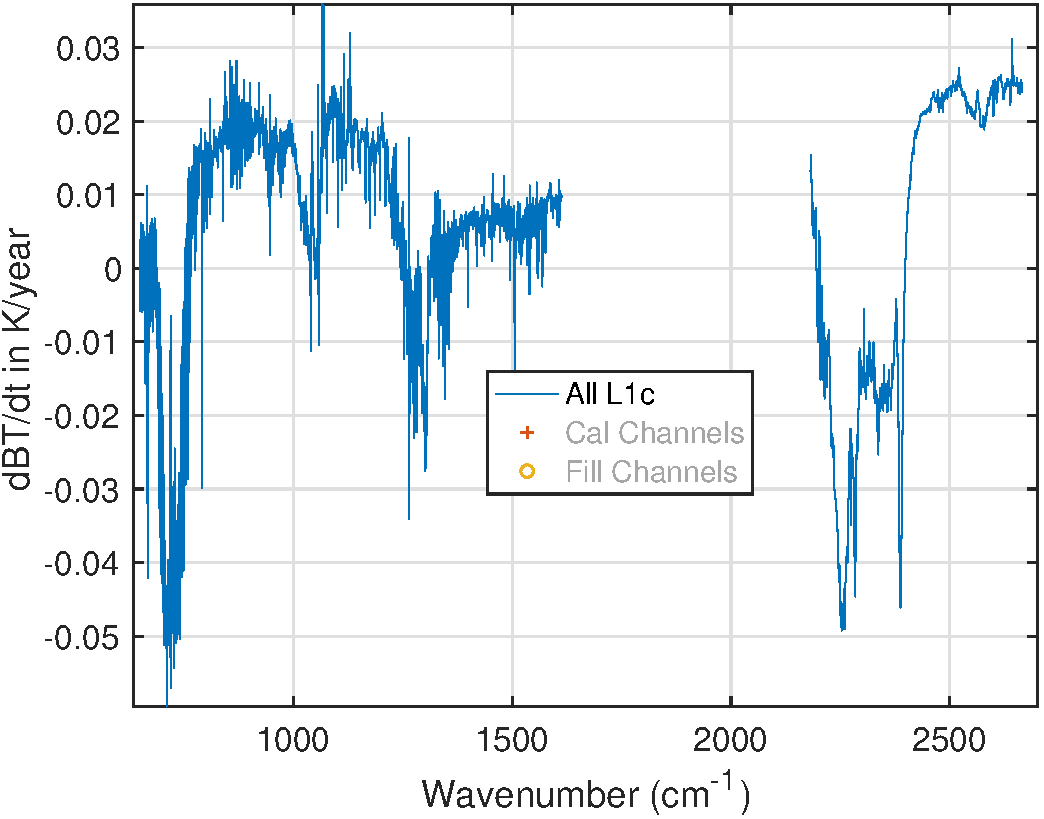
\includegraphics[width=0.85\linewidth]{./Figs/Pdf/rand_global_trend_l1c_overview.pdf}
\end{center}
\end{block}
\end{column}


\begin{column}{0.55\columnwidth}
\begin{block}{\footnotesize Fill channels marked}
\vspace{-0.1in}
\begin{center}
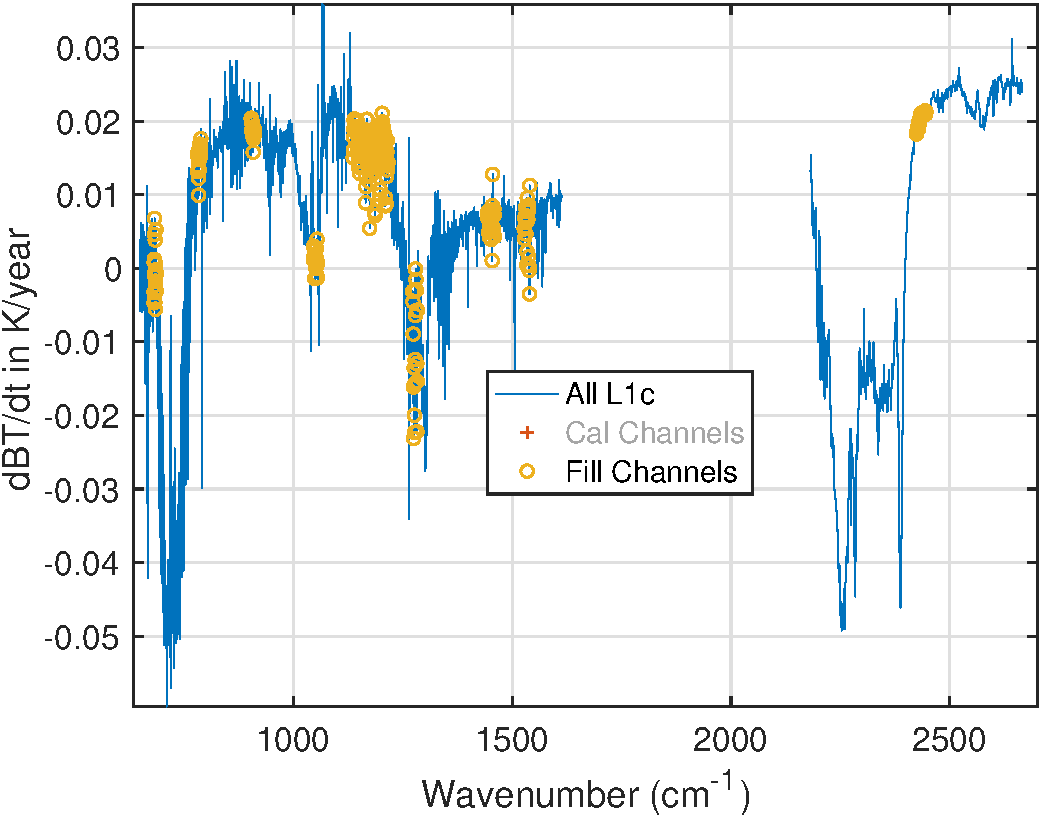
\includegraphics[width=0.85\linewidth]{./Figs/Pdf/rand_global_trend_l1c_overview_fill_marked.pdf}
\end{center}
\end{block}
\end{column}
\end{columns}


\vspace{-0.25in}

\begin{columns}
\begin{column}{0.55\columnwidth}
\begin{block}{\footnotesize Calibration channels}
\vspace{-0.1in}
\begin{center}
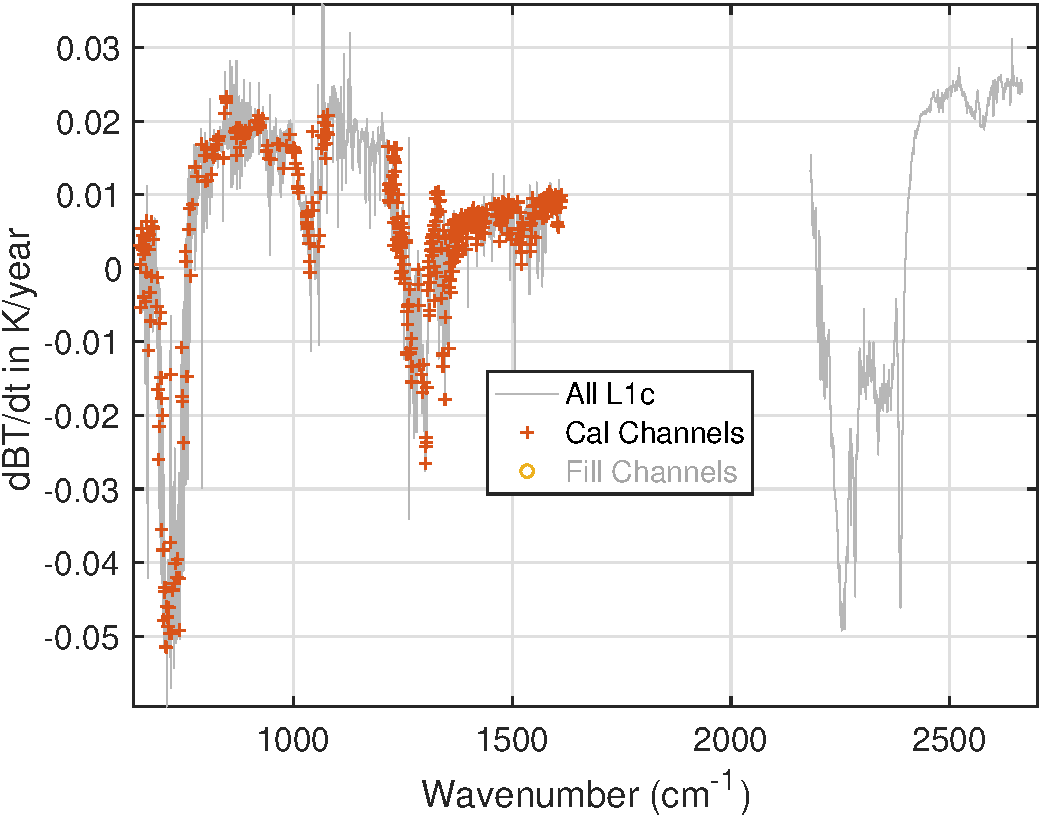
\includegraphics[width=0.75\linewidth]{./Figs/Pdf/rand_global_trend_l1c_overview_calfit_marked.pdf}
\end{center}
\end{block}
\end{column}


\begin{column}{0.55\columnwidth}
\begin{block}{\footnotesize}
\begin{footnotesize}
Channels used for calibration testing marked.\\
\vspace{0.05in}
These channels have no A/B state changes, good S/N, small drift\\
\vspace{0.05in}
Note sparsity of \cd channels in tropospheric sounding region\\
\end{footnotesize}
\end{block}
\end{column}
\end{columns}
\end{frame}

\begin{frame}[label={sec:orge78f532}]{\cd and \methane Trends Removed, Fitted Chans Only}
\vspace{-0.3in}
\begin{columns}
\begin{column}{0.55\columnwidth}
\begin{block}{\footnotesize AIRS + ERA}
\vspace{-0.1in}
\begin{center}
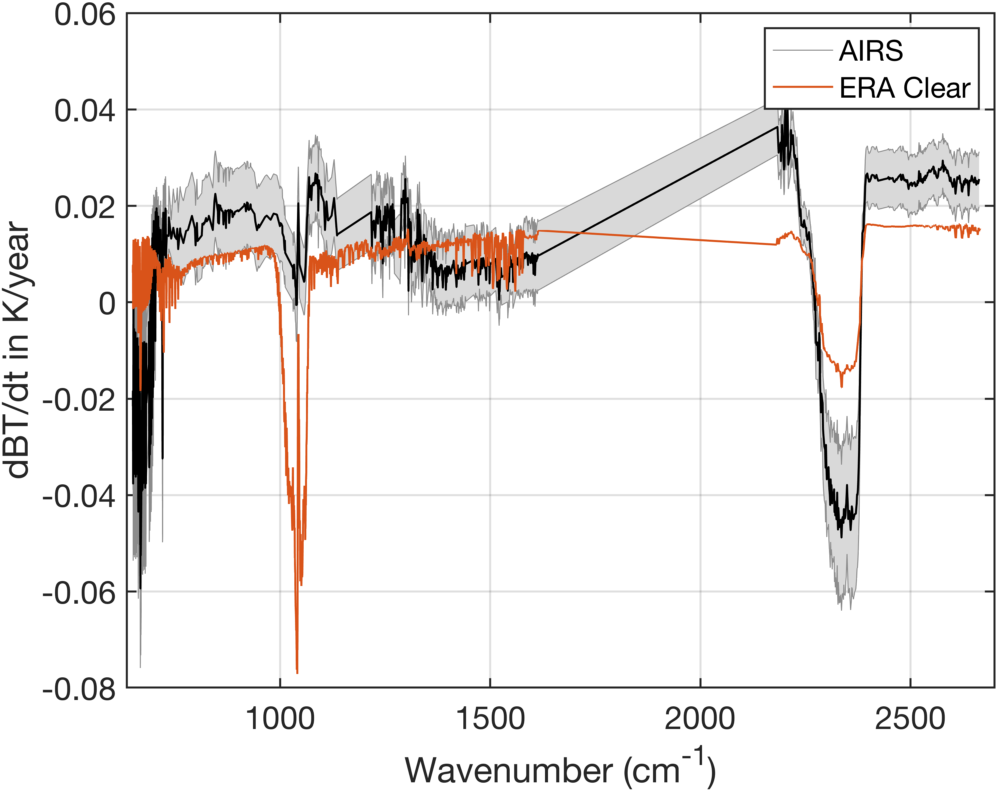
\includegraphics[width=\linewidth]{./Figs/Png/rand_global_trend_l1c_vs_era_clr_only_fit_chans.png}
\end{center}
\end{block}
\end{column}

\begin{column}{0.55\columnwidth}
\begin{block}{\footnotesize AIRS w/ 0.02K dT, RH constant}
\vspace{-0.1in}
\begin{center}
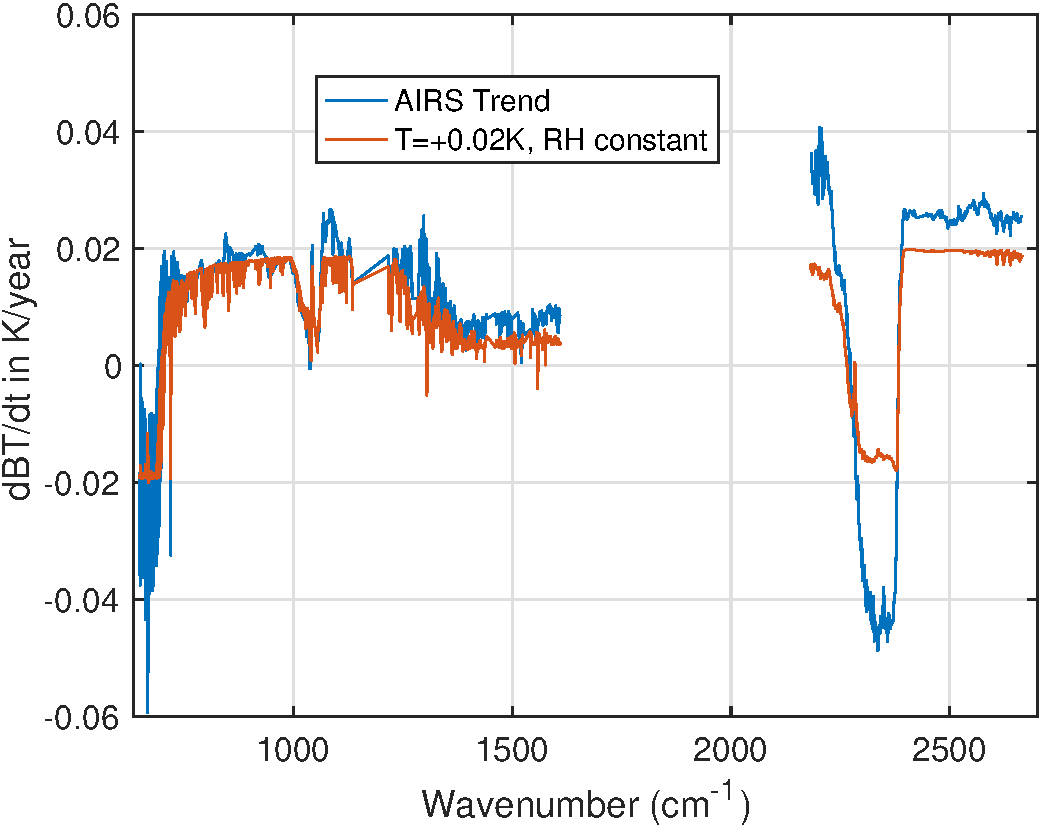
\includegraphics[width=\linewidth]{./Figs/Pdf/dbt_constantRH_dsurf_dtrop=0.02k_dstrat=m0.02k_withAIRS.pdf}
\end{center}
\end{block}
\end{column}
\end{columns}

\begin{small}
\begin{itemize}
\item Uncertainty (gray) is geophysical (Std over latitude).
\item RHS: Trop T(z) + 0.02K, Strat T(z) - 0.02K
\item \water trend is close to constant RH. (Varies with latitude).
\item Could suggest RH is a bit lower over time??
\item Shortwave appears to have a positive drift
\end{itemize}
\end{small}
\end{frame}

\begin{frame}[label={sec:orgc9dcc68}]{\small Switch to Clear Ocean Time Series: \cd Anomaly Fit for 20\textdegree{} N. (MLO)}
\vspace{-0.3in}
\begin{columns}
\begin{column}{0.55\columnwidth}
\begin{block}{\footnotesize Fitting Trick}
\begin{center}
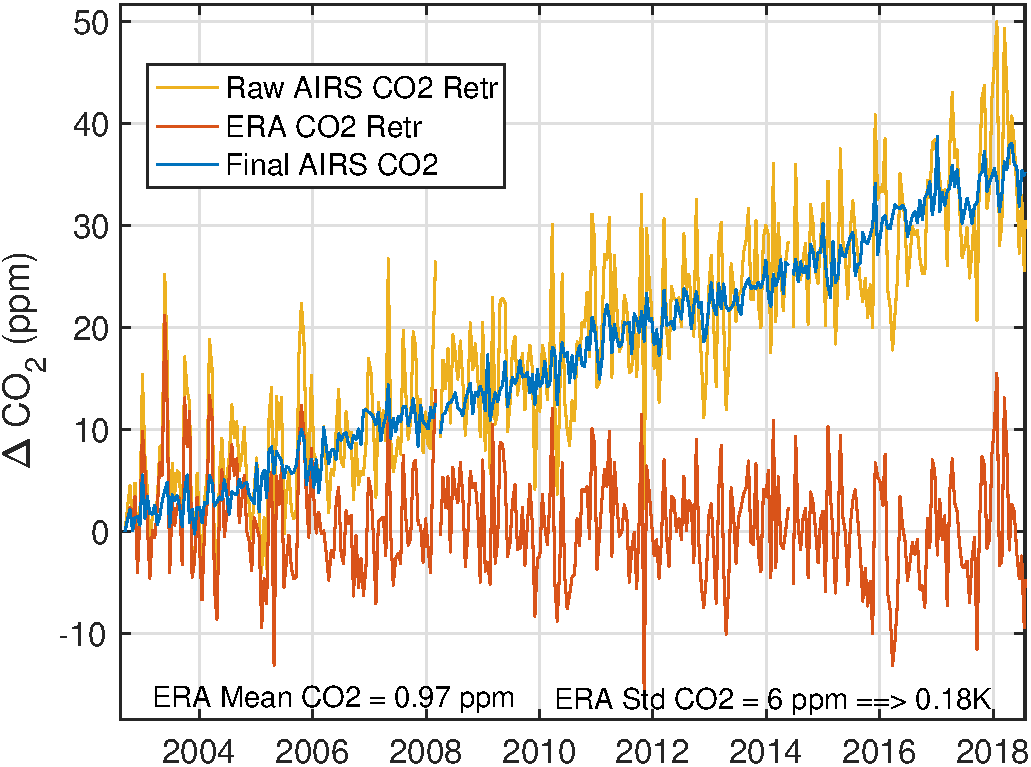
\includegraphics[width=\linewidth]{./Figs/Pdf/raw_co2_vs_era_co2_example_lati28_mlo_lat.pdf}
\end{center}
\end{block}
\end{column}

\begin{column}{0.55\columnwidth}
\begin{block}{\footnotesize Fitted \cd Anomalies}
\begin{center}
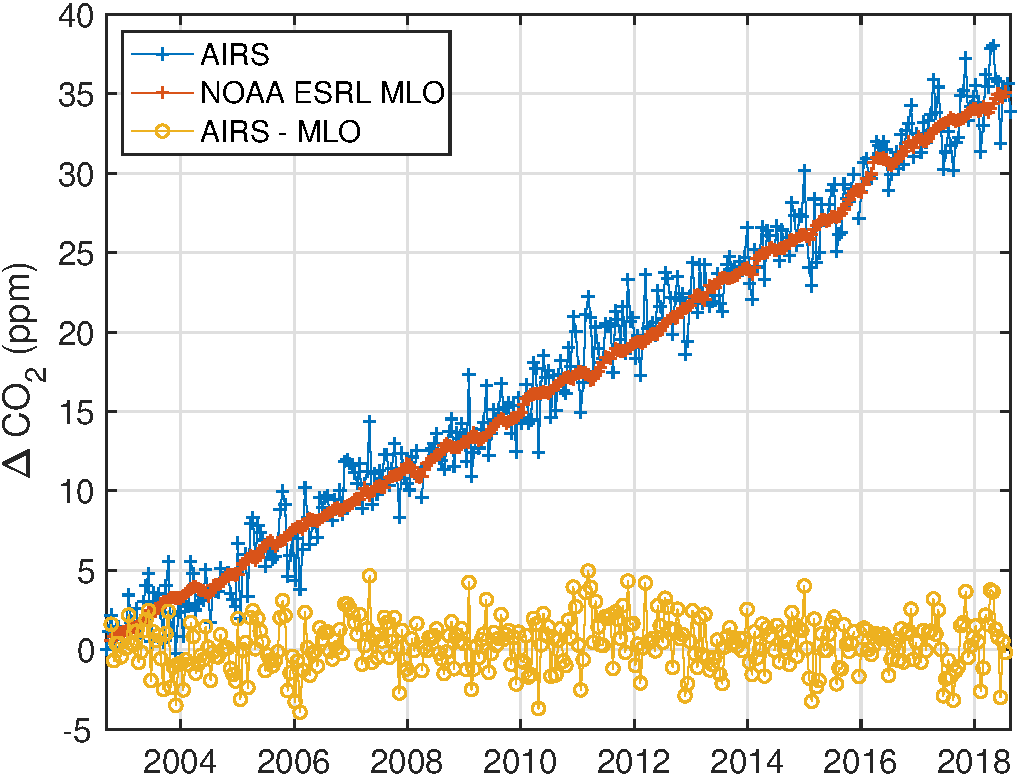
\includegraphics[width=\linewidth]{./Figs/Pdf/co2_airs_vs_mlo.pdf}
\end{center}
\end{block}
\end{column}
\end{columns}

\begin{footnotesize}
\begin{itemize}
\item ERA simulations done per footprint
\item Fit ERA simulation for \cd
\item Removes co-linearity? and lowers "noise"
\end{itemize}
\end{footnotesize}
\end{frame}

\begin{frame}[label={sec:orgcc0ebe8}]{\cd Anomaly Converted to B(T) Trends}
\begin{center}
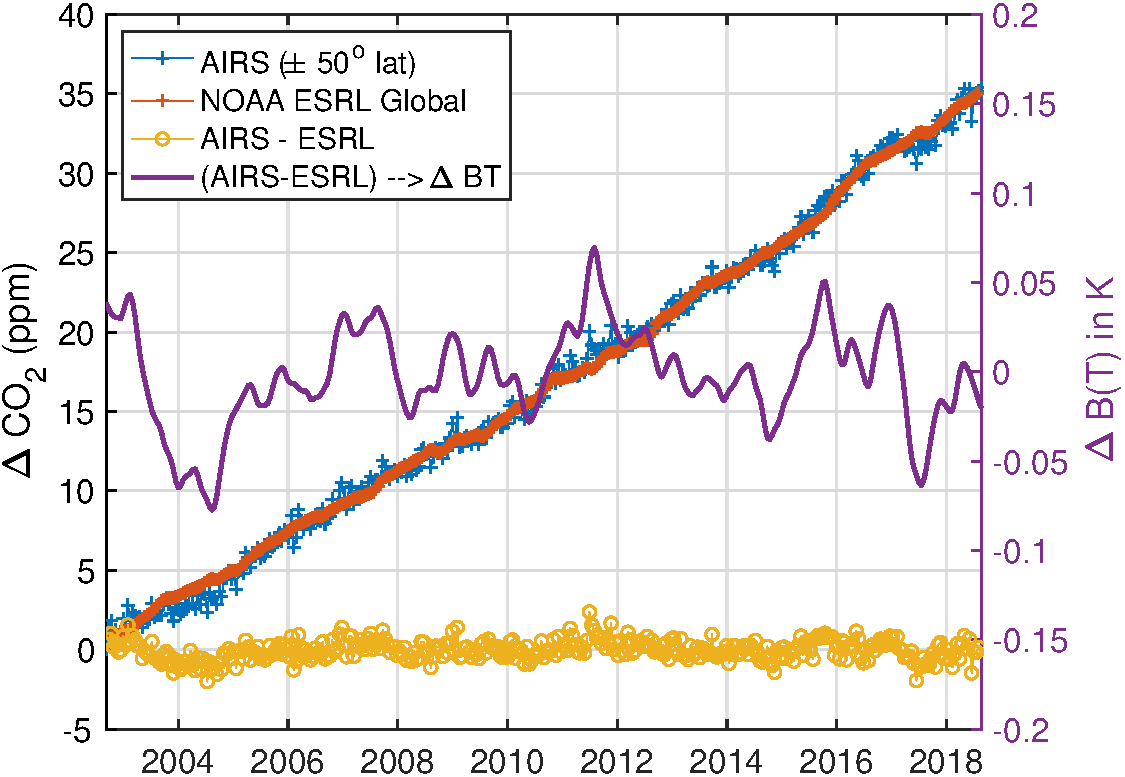
\includegraphics[width=0.7\linewidth]{./Figs/Pdf/co2_airs_vs_esrl_global_with_dbt.pdf}
\end{center}

\vspace{-0.1in}
\begin{footnotesize}
\begin{itemize}
\item Mean AIRS-ESRL \cd = 0.035 \textpm{} 0.032  pppm (1\(\sigma\) standard error)
\item Mean AIRS-ESRL in BT Units = +0.0026K \textpm{} 0.0023K (1\(\sigma\) standard error)
\item Sampling and ESRL errors hard to characterize
\item Suggests our \cd and SST channels are reasonably well-behaved
\item BUT: residuals of \cd sensitive channels do vary
\end{itemize}
\end{footnotesize}
\end{frame}


\begin{frame}[label={sec:org19445da}]{Other \cd Diagnostics}
\vspace{-0.35in}
\begin{columns}
\begin{column}{0.5\columnwidth}
\begin{block}{\footnotesize Growth Rates}
\vspace{-0.1in}
\begin{center}
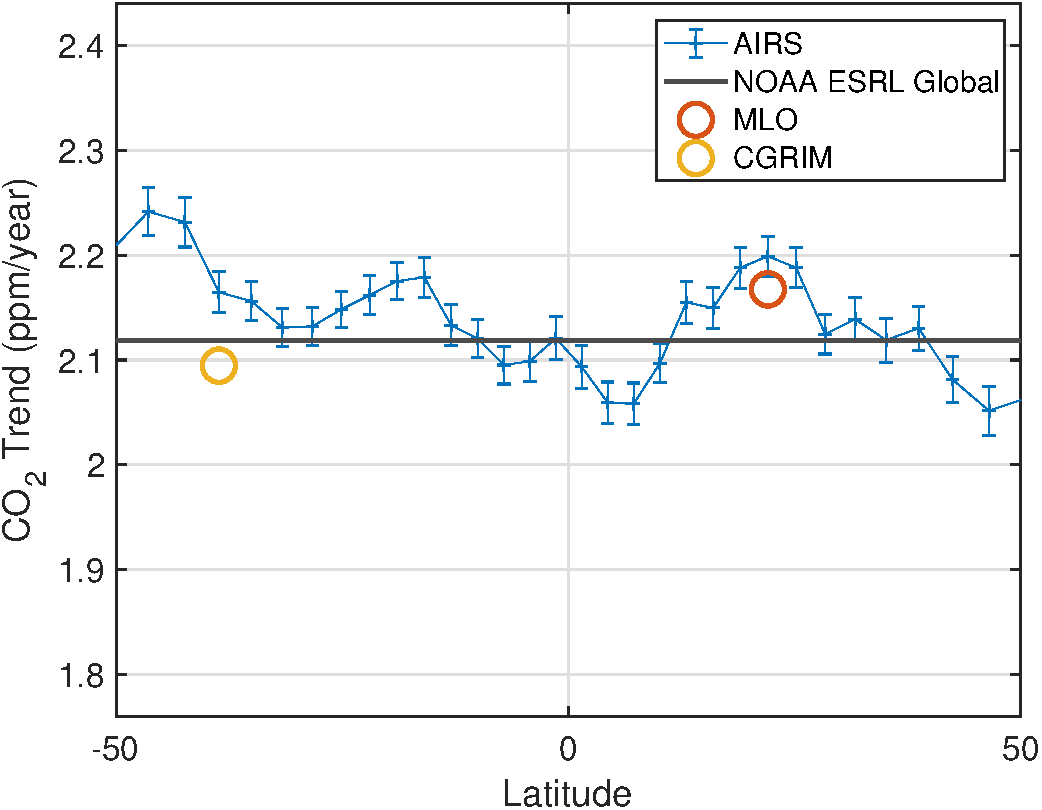
\includegraphics[width=0.9\linewidth]{./Figs/Pdf/co2_growth_vs_lat.pdf}
\end{center}
\end{block}
\end{column}

\begin{column}{0.5\columnwidth}
\begin{block}{\footnotesize Growth Rate Anomaly}
\vspace{-0.1in}
\begin{center}
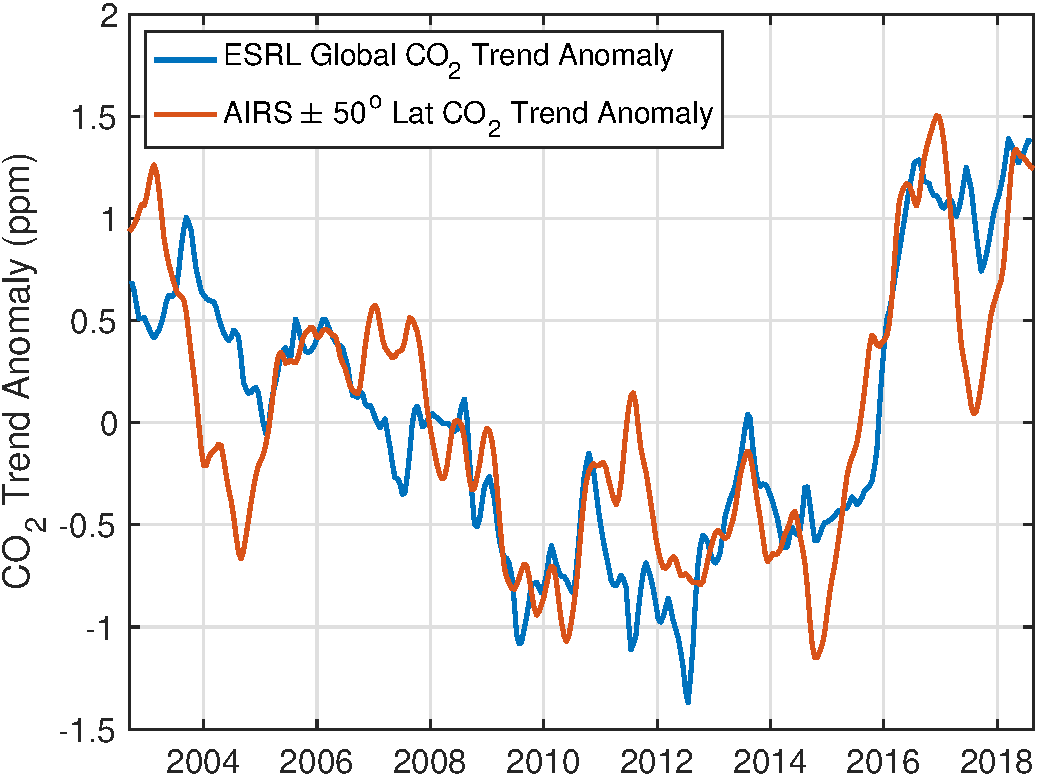
\includegraphics[width=0.9\linewidth]{./Figs/Pdf/co2_airs_vs_esrl_global_growth_anom.pdf}
\end{center}
\end{block}
\end{column}
\end{columns}

\vspace{-0.2in}

\begin{columns}
\begin{column}{0.5\columnwidth}
\begin{block}{\footnotesize Zonal Anomalies}
\vspace{-0.1in}
\begin{center}
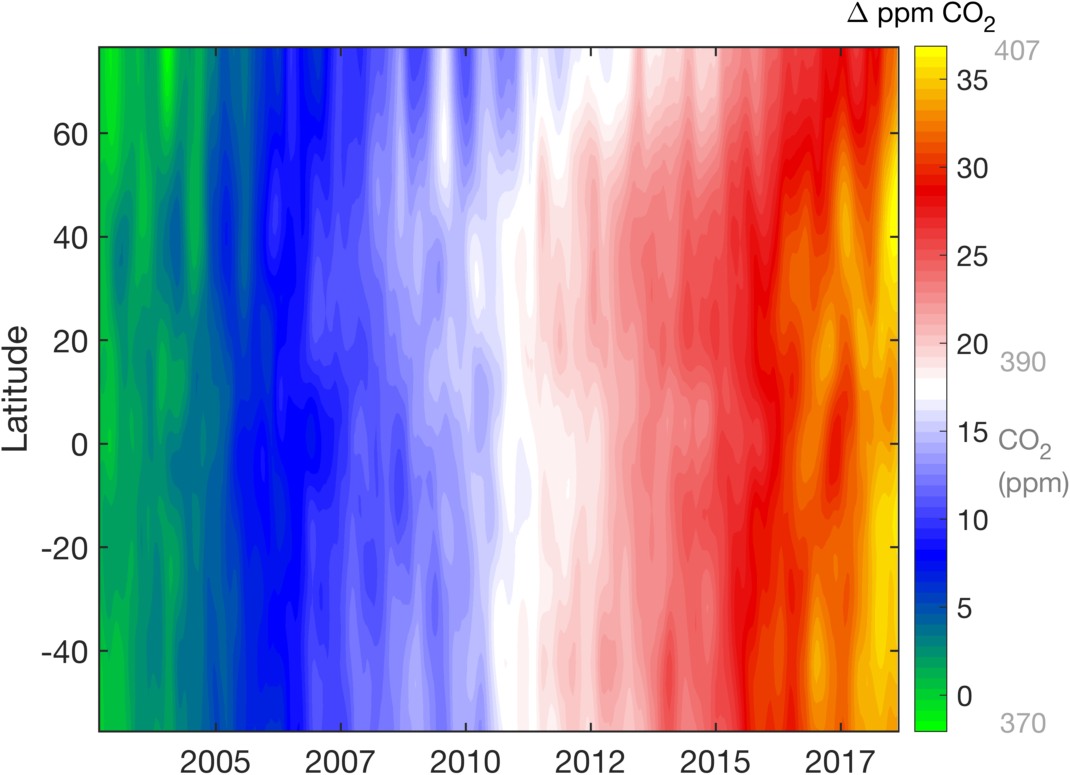
\includegraphics[width=0.9\linewidth]{./Figs/Png/co2_anom_image_lat_vs_time.png}
\end{center}
\end{block}
\end{column}

\begin{column}{0.5\columnwidth}
\begin{block}{}
\vspace{-0.2in}
\begin{footnotesize}
\begin{itemize}
\item Growth rate anomaly accuracy very encouraging.
\item AIRS - Avg(MLO + CGRIM) growth rate difference: -0.0056K/year in BT units
\item MLO, CGRIM growth rate uncertainty from ESRL \textasciitilde{}0.0051K/year
\end{itemize}
\end{footnotesize}
\end{block}
\end{column}
\end{columns}
\end{frame}
\begin{frame}[label={sec:orgda3882b}]{\nitrous Retrieved Anomalies}
\begin{center}
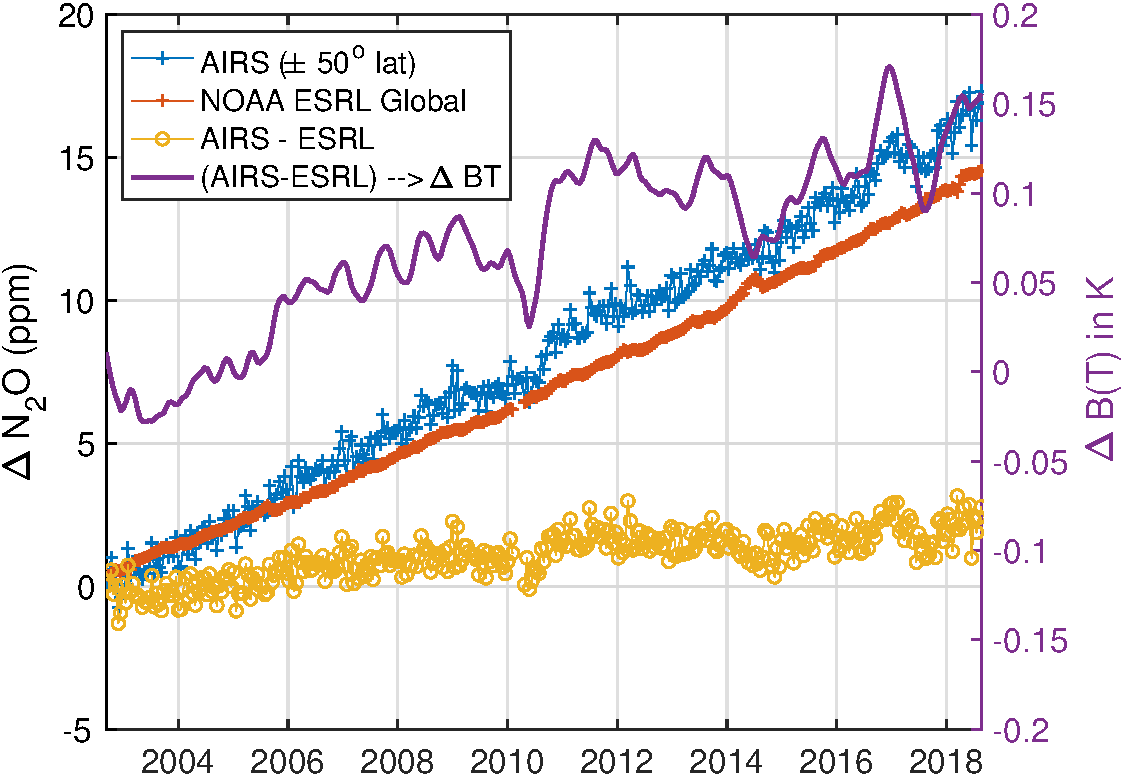
\includegraphics[width=0.7\linewidth]{./Figs/Pdf/n2o_airs_vs_esrl_global_with_dbt.pdf}
\end{center}

\begin{footnotesize}
\begin{itemize}
\item This is what we are after
\item Something a little before 2006?
\item A jump due to the Jan. 2010 shutdown
\item Stable otherwise
\item Look at residuals of fits to understand guilty channels
\end{itemize}
\end{footnotesize}
\end{frame}

\begin{frame}[label={sec:orga13fbe5}]{\methane Retrieved Anomalies}
\begin{center}
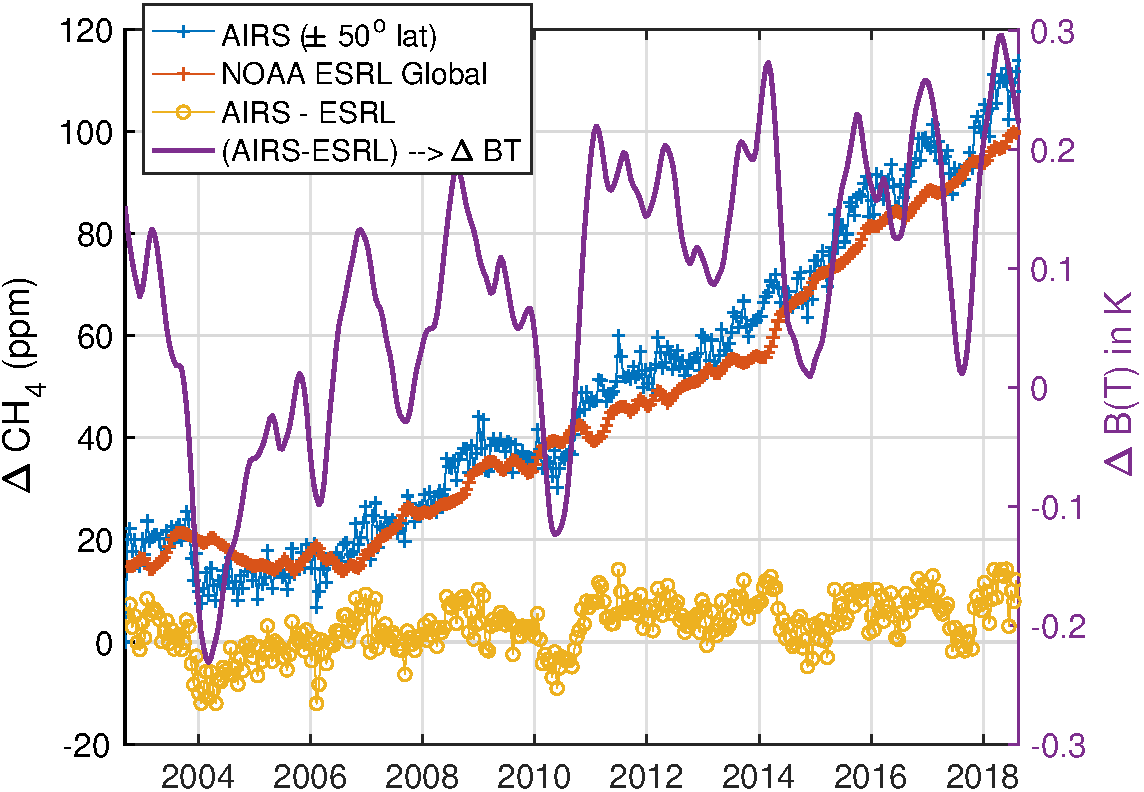
\includegraphics[width=0.7\linewidth]{./Figs/Pdf/ch4_airs_vs_esrl_global_with_dbt.pdf}
\end{center}

\begin{footnotesize}
\begin{itemize}
\item Is \methane well mixed enough for this analysis?
\item Clearly an offset in Jan 2010 but it recovered (seen in spectral!)
\item Clear Nov. 2003 B(T) shift
\end{itemize}
\end{footnotesize}
\end{frame}

\begin{frame}[label={sec:orgd4f41f5}]{\methane Growth Rate Anomalies}
\begin{center}
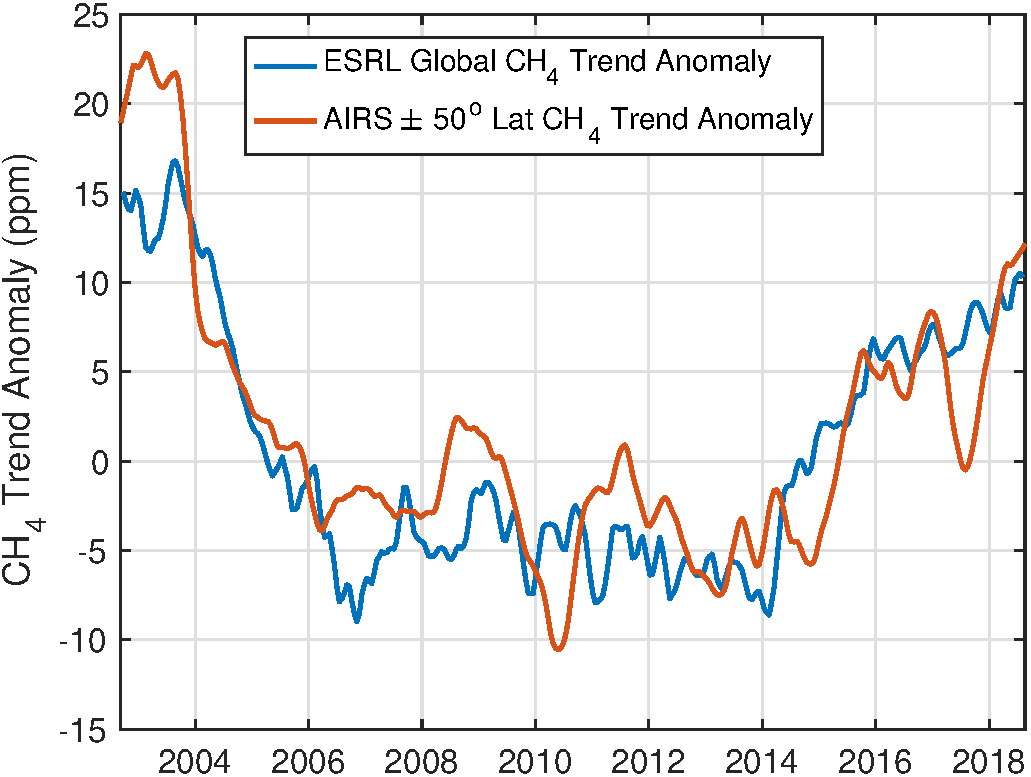
\includegraphics[width=0.7\linewidth]{./Figs/Pdf/ch4_airs_vs_esrl_global_growth_anom.pdf}
\end{center}

\begin{footnotesize}
\begin{itemize}
\item Very nice agreement with NOAA ESRL in-situ
\item Shows drop-off in global \methane growth early in mission
\item Then increasing growth starting in 2014
\end{itemize}
\end{footnotesize}
\end{frame}

\begin{frame}[label={sec:orgc33163f}]{Unlike Retrievals We'd Like to Examine Many Channels}
\vspace{-0.3in}

\begin{columns}
\begin{column}{0.55\columnwidth}
\begin{block}{\footnotesize IASI: 11-Year Trend}
\vspace{-0.1in}
\begin{center}
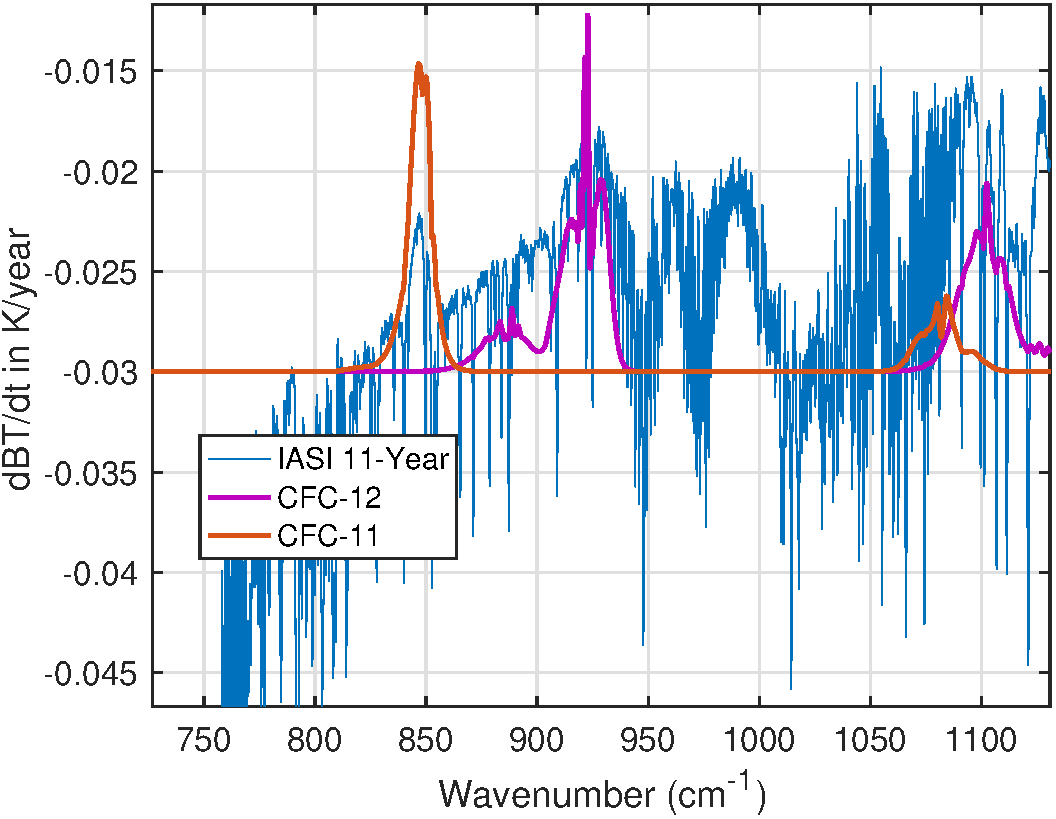
\includegraphics[width=0.75\linewidth]{./Figs/Pdf/iasi_cfc_signatures.pdf}
\end{center}
\end{block}
\end{column}

\begin{column}{0.55\columnwidth}
\begin{block}{\footnotesize}
\begin{footnotesize}
That means taking the CFC 11 and 12 into account.\\
\vspace{0.05in}
Maybe 3 strong CFC 11 channels?\\
\vspace{0.05in}
Maybe 3-5 strong CFC 12 channels?\\
\vspace{0.05in}
But, need to remove effects in wings
\end{footnotesize}
\end{block}
\end{column}
\end{columns}

\vspace{-0.25in}

\begin{columns}
\begin{column}{0.55\columnwidth}
\begin{block}{\footnotesize IASI Trend Zoom}
\vspace{-0.1in}
\begin{center}
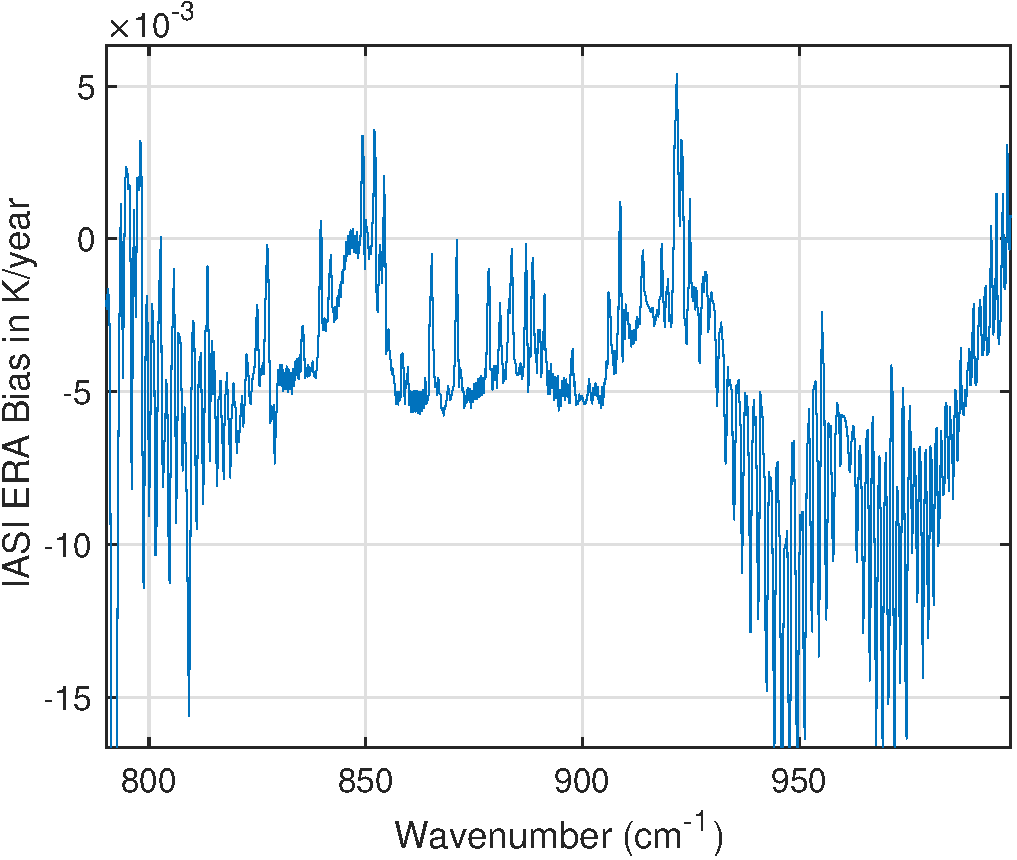
\includegraphics[width=0.75\linewidth]{./Figs/Pdf/iasi_cfc_bias.pdf}
\end{center}
\end{block}
\end{column}

\begin{column}{0.55\columnwidth}
\begin{block}{\footnotesize AIRS Trend Zoom}
\begin{center}
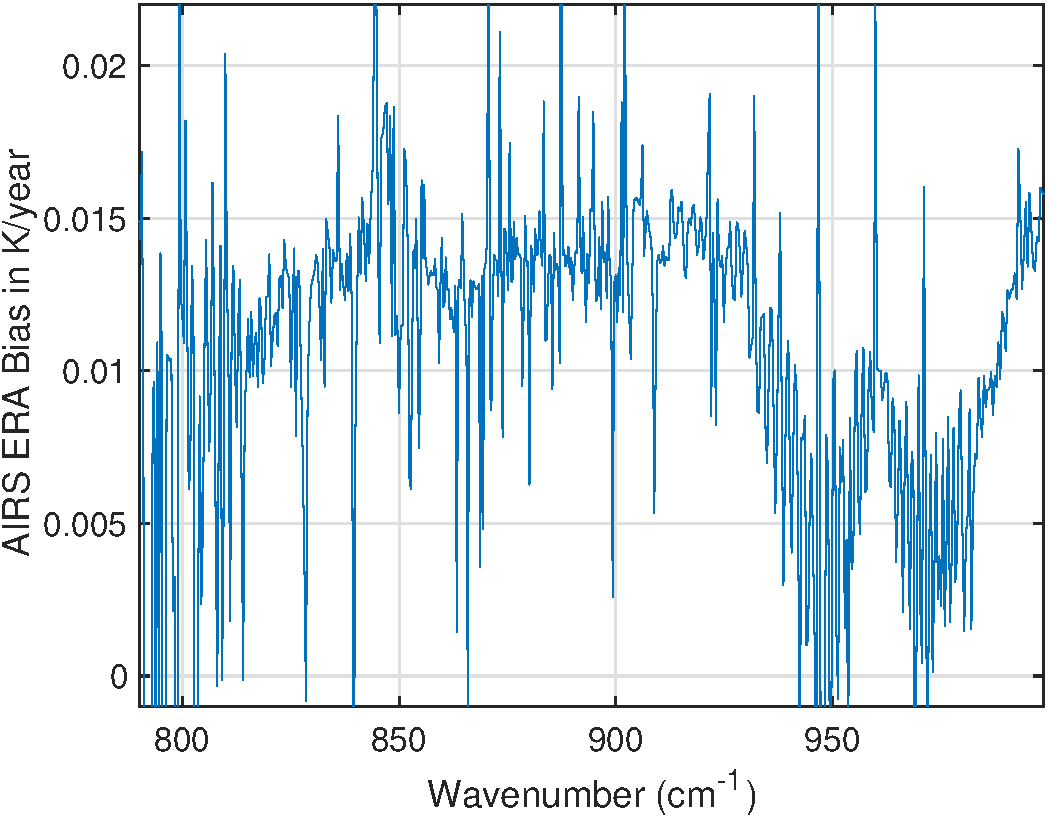
\includegraphics[width=0.75\linewidth]{./Figs/Pdf/airs_cfc_bias_iasi_times.pdf}
\end{center}
\end{block}
\end{column}
\end{columns}
\end{frame}

\begin{frame}[label={sec:org421ec84}]{Fit to AIRS CFC-11 for Removal in Fit Residuals}
\vspace{-0.3in}
\begin{columns}
\begin{column}{0.55\columnwidth}
\begin{block}{\footnotesize CFC-11 B(T) Trend}
\vspace{-0.1in}
\begin{center}
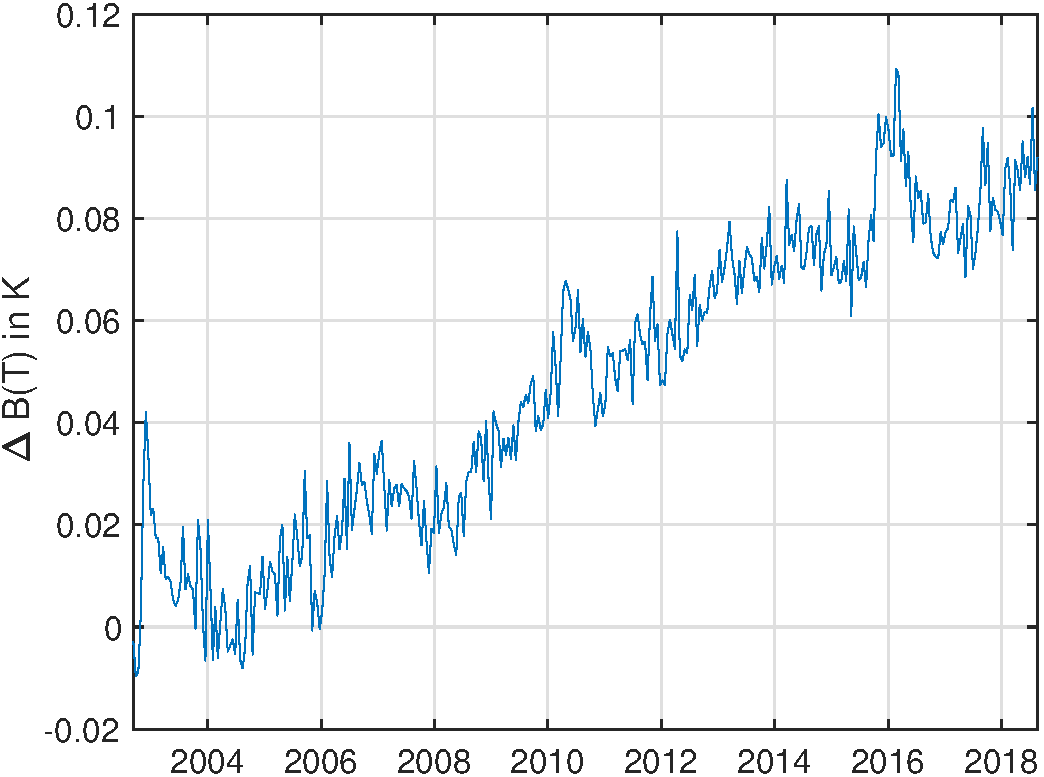
\includegraphics[width=0.85\linewidth]{./Figs/Pdf/cfc11_bt_trend.pdf}
\end{center}
\end{block}
\end{column}

\begin{column}{0.55\columnwidth}
\begin{block}{\footnotesize CFC ppb Trend}
\vspace{-0.1in}
\begin{center}
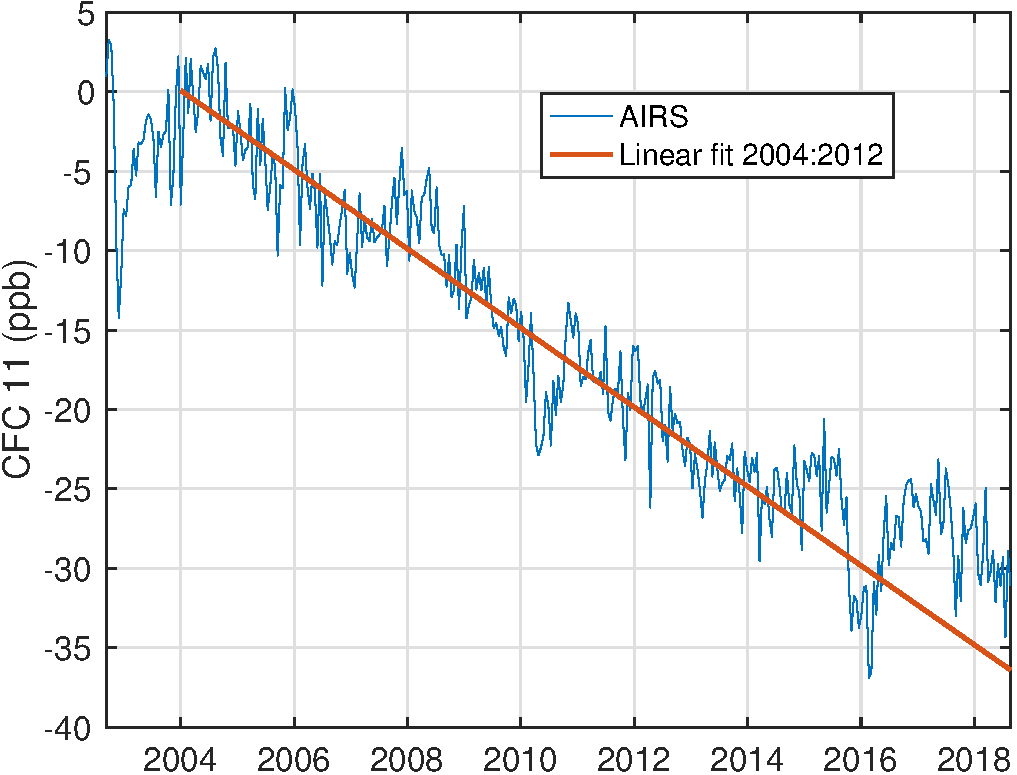
\includegraphics[width=0.85\linewidth]{./Figs/Pdf/cfc11_trend.pdf}
\end{center}
\end{block}
\end{column}
\end{columns}

\begin{footnotesize}
\begin{itemize}
\item Reasonably linear negative trend, as expected
\item Values agree well with in-situ
\item BUT, the trend appears to be decreasing!
\item Also expected from in-situ: possible cause is Chinese production of CFC-11
\item ENSO signals in time series: retrieval problem or something real?
\item Clear problems due to Nov. 2003 AQUA shutdown
\end{itemize}
\end{footnotesize}
\end{frame}
\begin{frame}[label={sec:org89b3cbb}]{SST Retrieved from Anomaly Fits}
\begin{center}
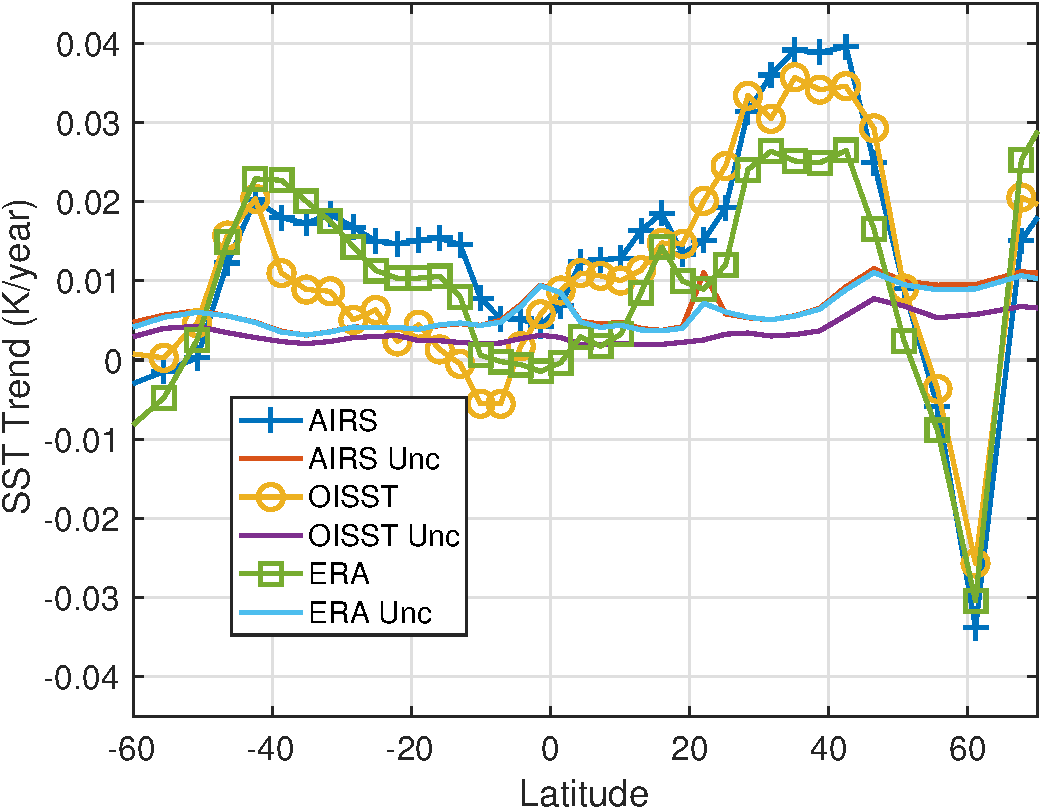
\includegraphics[width=0.7\linewidth]{./Figs/Pdf/co2_anom_sst_vs_oisst_clear_sampled_and_era.pdf}
\end{center}
\begin{footnotesize}
\begin{itemize}
\item OISST likely better?  AIRS-OISST = +0.005 \textpm{} 0.007 K/year (tropics)
\item ERA transitioned from RTG to OSTIA in Feb. 2009, we likely see that
\item Differences very small and at limits of SST climatologies
\end{itemize}
\end{footnotesize}
\end{frame}

\begin{frame}[label={sec:org7d021c3}]{OE Fit Residuals:  Main Diagnostic of Trends}
\vspace{-0.1in}
\begin{center}
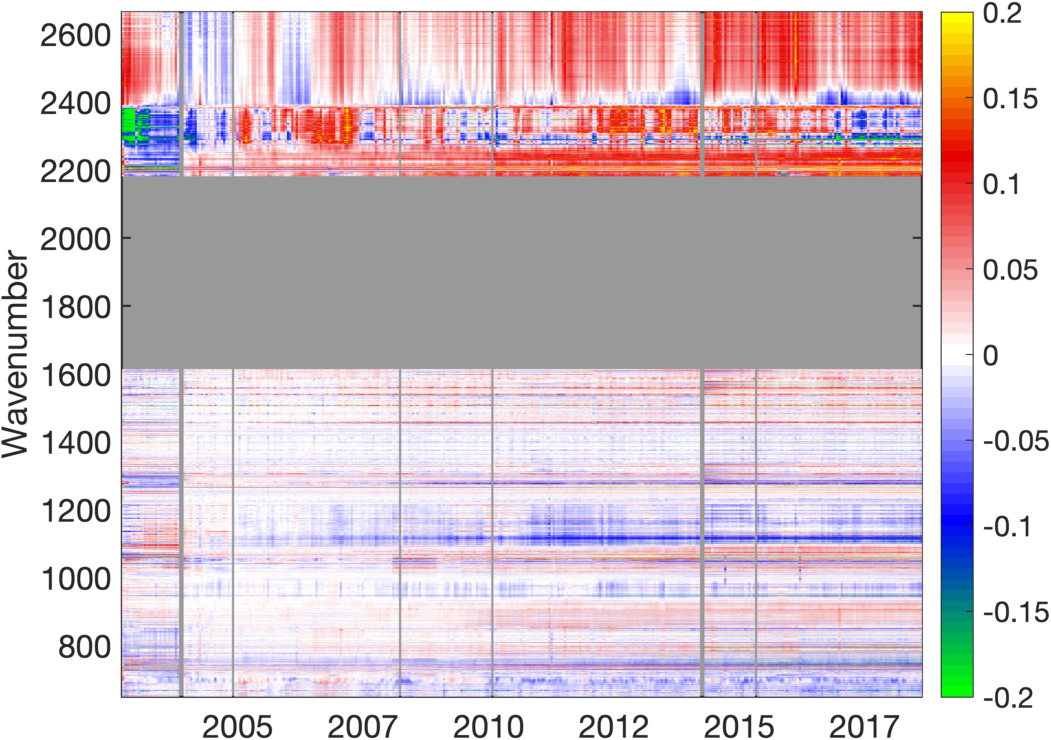
\includegraphics[width=0.7\linewidth]{./Figs/Png/best_co2_anom_resid.png}
\end{center}

\vspace{-0.1in}
\begin{footnotesize}
\begin{itemize}
\item All residuals shown (including fill)
\item Color scale is \(\Delta\) BT in K
\item \textpm{} full scale equivalent to \textpm{} 0.0125K/year drift
\item Remember: we would like to get to the 0.003K/year level or better
\item Easy to see issues: Shortwave!!, Nov. 2003, some bad arrays, etc.
\end{itemize}

\end{footnotesize}
\end{frame}

\begin{frame}[label={sec:orga34d887}]{Zoom of Residual w/o Shortwave}
\begin{center}
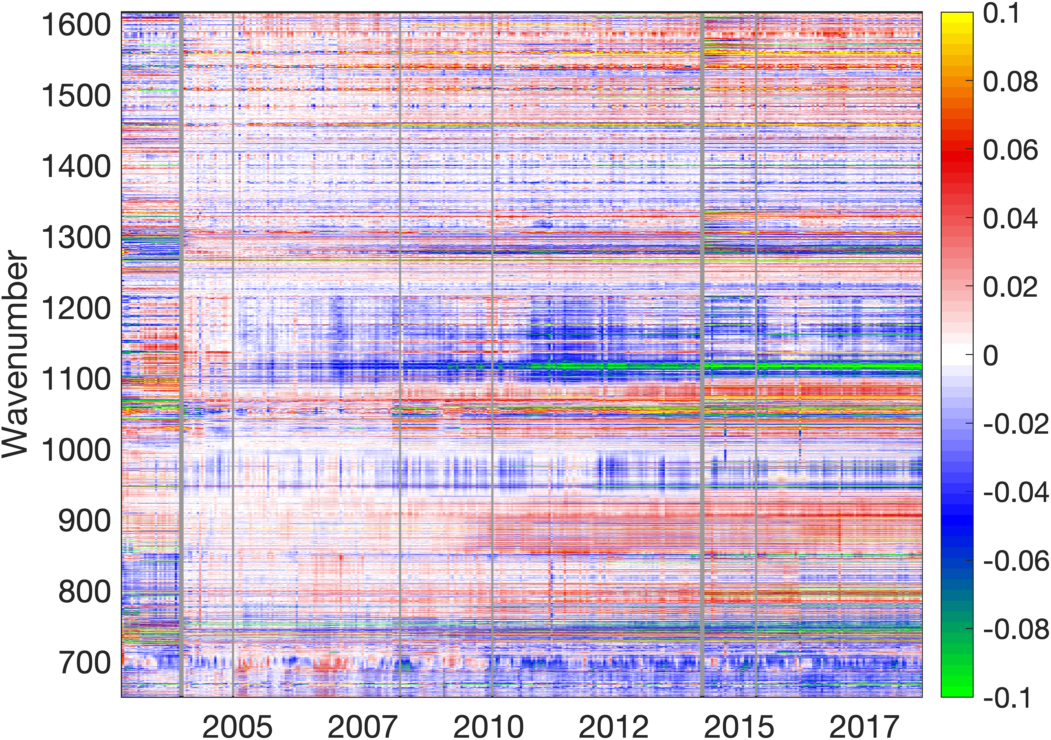
\includegraphics[width=0.8\linewidth]{./Figs/Png/best_co2_anom_resid_no_sw.png}
\end{center}

\begin{itemize}
\item Note: colorscale now \textpm{} 0.1 K
\item But, only limited usefulness if fitted geophysical parameters are good!
\end{itemize}
\end{frame}

\begin{frame}[label={sec:org14a943c}]{Deep Convective Cloud Time Series}
\vspace{-0.35in}

\begin{columns}
\begin{column}{0.5\columnwidth}
\begin{block}{\footnotesize AIRS vs IASI Time Series}
\vspace{-0.1in}
\begin{center}
\includegraphics[width=\linewidth]{./Figsdc/Pdf/bt2616_and_bt960_dcc_vs_time_airs_and_iasi.pdf}
\end{center}
\end{block}
\end{column}

\begin{column}{0.5\columnwidth}
\begin{block}{\footnotesize Trends (A/B detector issues)}
\vspace{-0.1in}
\begin{center}
\includegraphics[width=\linewidth]{./Figsdc/Pdf/airs_iasi_dcc_rate_lw_ab_diffs_vs_iasi.pdf}
\end{center}
\end{block}
\end{column}
\end{columns}

\vspace{-0.1in}
\begin{footnotesize}
\begin{itemize}
\item Shortwave drift 2004-2012
\item Consistent with Space Look getting colder
\item Back of the envelope: 
\begin{itemize}
\item at 210K dBT/dyr = 0.47K/ for 2616 \wn
\item at 300K equivalent to 0.0045K/year!
\item at 255/265K (Arctic) equivalent to 0.30/0.19 K/decade
\end{itemize}
\end{itemize}

\end{footnotesize}
\end{frame}

\begin{frame}[label={sec:org7365180}]{Sample Fit Residual Time Series}
\vspace{-0.35in}
\begin{columns}
\begin{column}{0.5\columnwidth}
\begin{block}{\footnotesize Water Vapor Channels}
\vspace{-0.1in}
\begin{center}
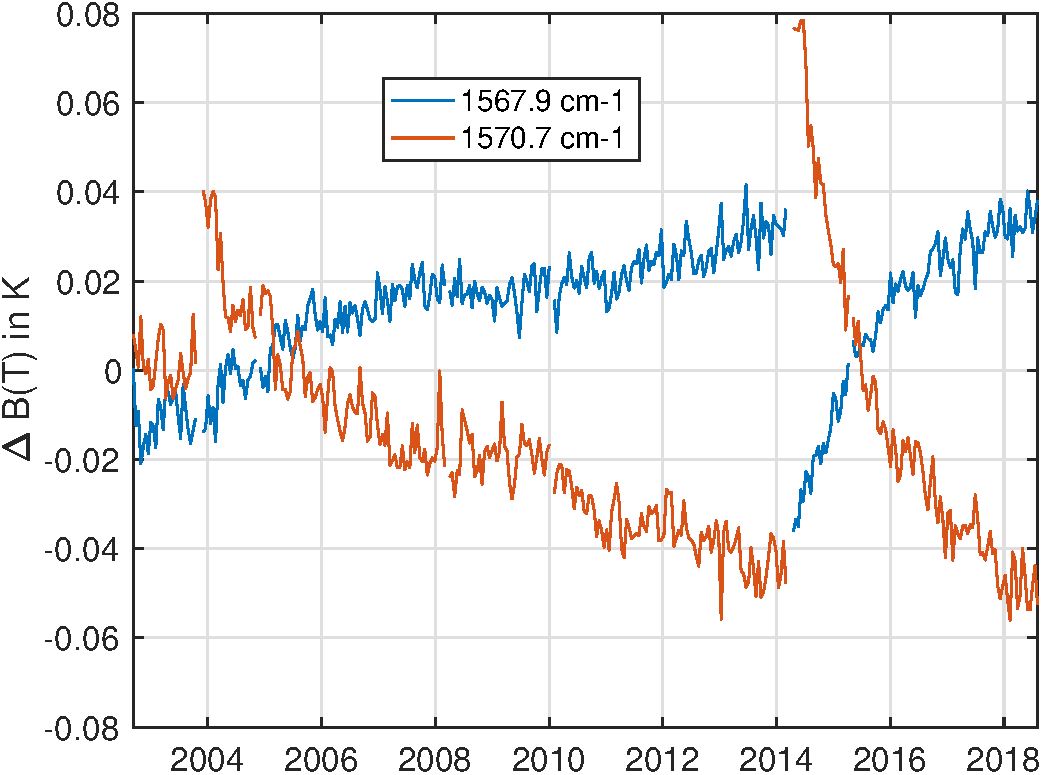
\includegraphics[width=0.85\linewidth]{./Figs/Pdf/resid_1567_and_1570_cm01_dnu.pdf}
\end{center}
\end{block}
\end{column}

\begin{column}{0.5\columnwidth}
\begin{block}{\footnotesize Effect of Nov. 2003 Shutdown}
\vspace{-0.1in}
\begin{center}
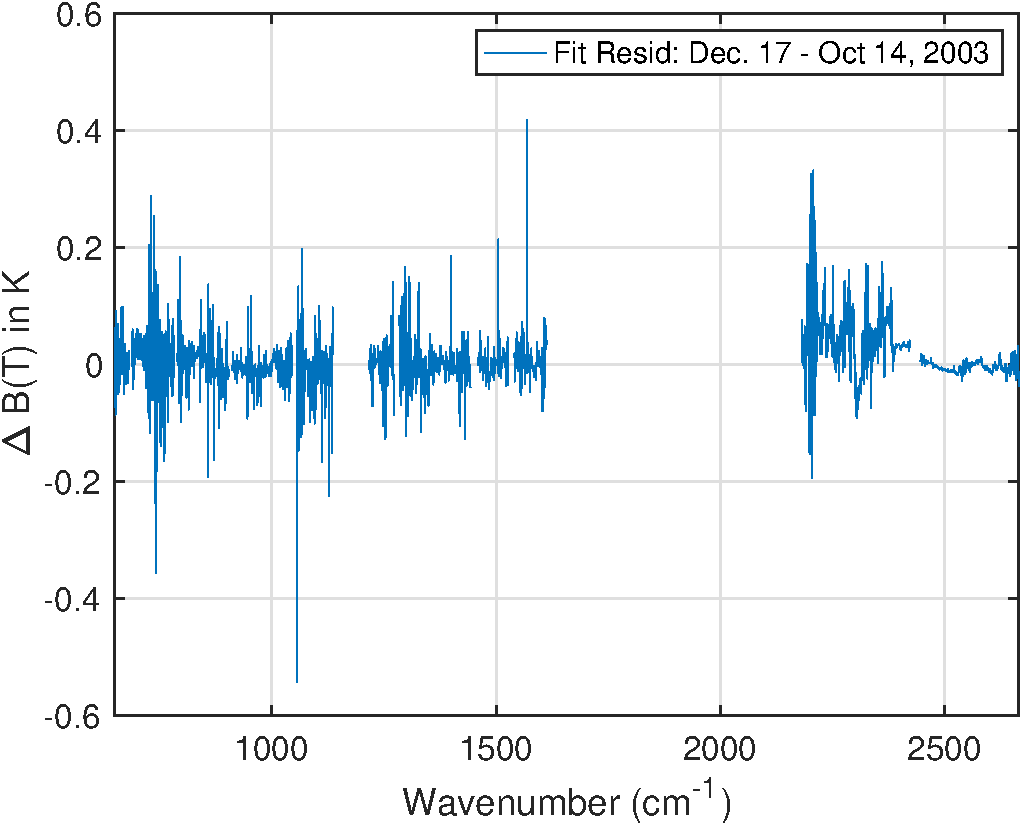
\includegraphics[width=0.85\linewidth]{./Figs/Pdf/resid_spectrum_dec17_minus_oct14_2003.pdf}
\end{center}
\end{block}
\end{column}
\end{columns}

\vspace{-0.2in}

\begin{columns}
\begin{column}{0.5\columnwidth}
\begin{block}{}
\begin{footnotesize}
\begin{itemize}
\item AIRS "events" easily seen
\item Fix events, re-retrieve \cd, SST, etc. and test
\item FUTURE: Use DCC spectra instead of clear for scene dependence
\end{itemize}
\end{footnotesize}
\end{block}
\end{column}

\begin{column}{0.5\columnwidth}
\begin{block}{\footnotesize Zoom of Nov. 2003 Shutdown (fringes)}
\vspace{-0.1in}
\begin{center}
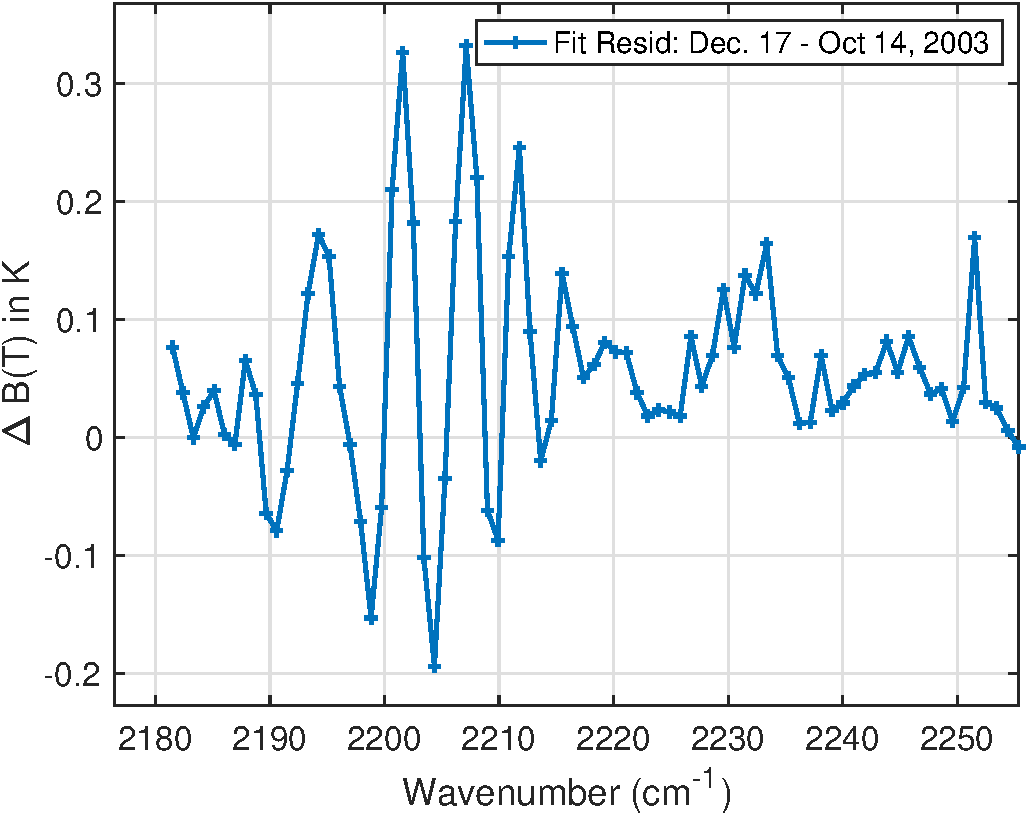
\includegraphics[width=0.85\linewidth]{./Figs/Pdf/resid_spectrum_dec17_minus_oct14_2003_swzoom.pdf}
\end{center}
\end{block}
\end{column}
\end{columns}
\end{frame}

\begin{frame}[label={sec:org2489db7}]{Summary}
\begin{itemize}
\item Validate OE retrieval products (done above)
\item Adjust channel "event" offsets
\item Re-do OE retrievals, re-validated.
\item Add more channels as they are "fixed"
\item etc.
\end{itemize}

\begin{block}{Improvements Possible}
\begin{itemize}
\item More uniform sampling of clear
\item Must add colder scenes (DCC's) to process since adjustments are likely scene temperature dependent
\item OE can always be improved, start to look at T(z), \water(z), \ozone(z) profile retrievals once have more uniform (gridded) sampling.
\end{itemize}
\end{block}
\end{frame}

\begin{frame}[label={sec:orga863315}]{SW Fit Residual Trends: Impact on Warming Estimates}
\begin{columns}
\begin{column}{0.6\columnwidth}
\begin{block}{}
\vspace{-0.3in}
\begin{center}
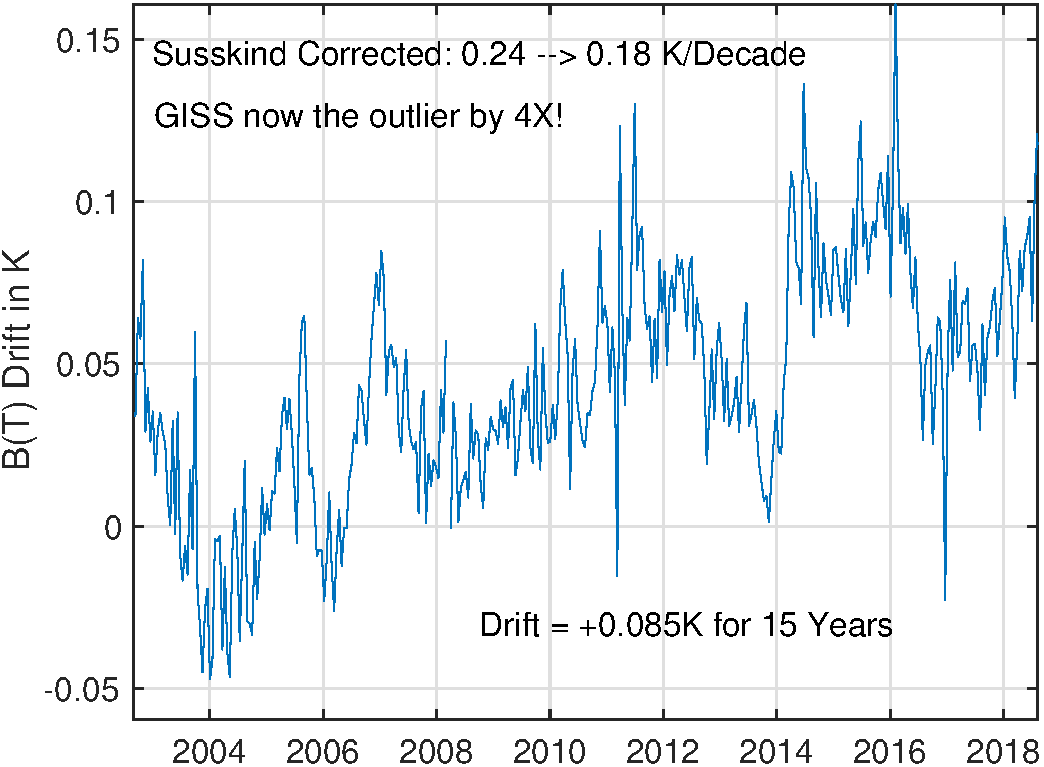
\includegraphics[width=\linewidth]{./Figs/Pdf/bt_drift_from_anom_resid_2613_chan_v2.pdf}
\end{center}
\end{block}
\end{column}

\begin{column}{0.4\columnwidth}
\begin{block}{From Susskind et. al.}
\begin{small}
\begin{center}
\begin{tabular}{ll}
AIRS & 0.24 \textpm{} 0.12\\
AIRS Corrected & 0.18\\
GISTEMP & 0.22 \textpm{} 0.13\\
HadCRUT4 & 0.17 \textpm{} 0.13\\
C\&W & 0.19 \textpm{} 0.12\\
ECMWF & 0.20 \textpm{} 0.16\\
UAH LT & 0.18\\
\end{tabular}
\end{center}
\end{small}
\end{block}
\end{column}
\end{columns}

Shortwave drift correction reduces AIRS global temperature trend by 33\% and bring AIRS into close agreement with HadCRUT4, C\&W, and UAH LT, significantly worse agreement with GISTEMP.

\vspace{-0.1in}
\end{frame}

\begin{frame}[label={sec:org540bbdf}]{Latitude Dependence Surface Trends}
\vspace{-0.35in}
\begin{columns}
\begin{column}{0.55\columnwidth}
\begin{block}{\footnotesize Susskind 2019: SW}
\vspace{-0.15in}
\begin{center}
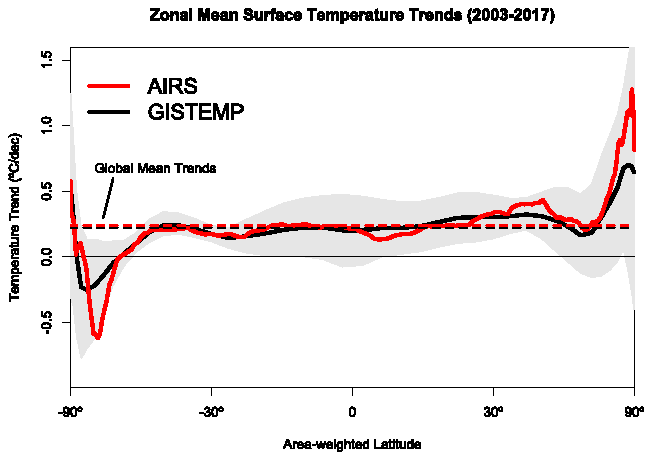
\includegraphics[width=\linewidth]{./Figs/Pdf/susskind_giss_trend_vs_lat.pdf}
\end{center}
\end{block}
\end{column}

\begin{column}{0.55\columnwidth}
\begin{block}{\footnotesize UMBC Trends: LW and SW}
\begin{center}
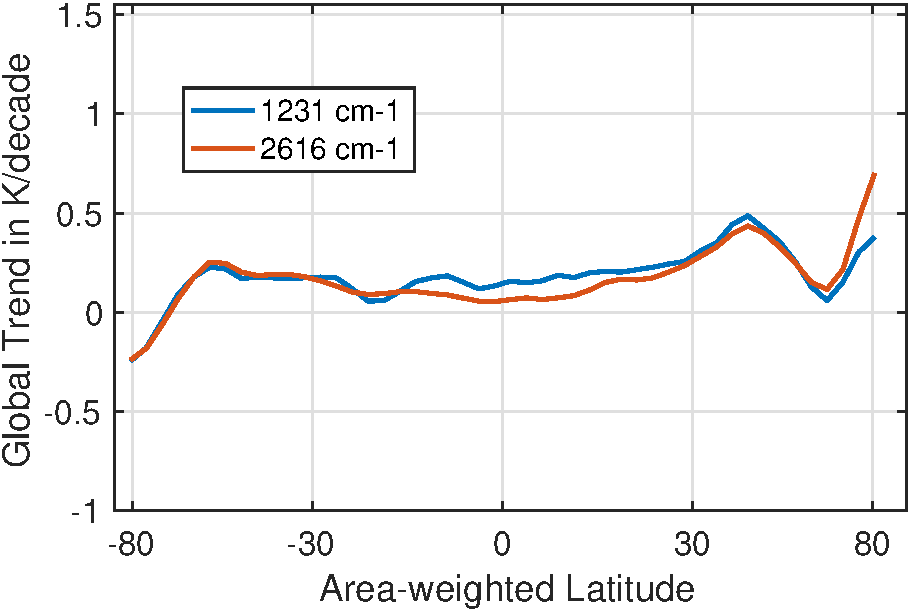
\includegraphics[width=\linewidth]{./Figs/Pdf/bt_global_trend_area_weight_lat_1231_vs_2616_from_hottest_v2.pdf}
\end{center}
\end{block}
\end{column}
\end{columns}

\vspace{-0.15in}
\begin{footnotesize}
Global Means
\vspace{-0.1in}
\begin{center}
\begin{tabular}{rrrrr}
GISS & Susskind & UMBC-1231 & UMBC-2616 & HadCRUT4\\
0.22 & 0.24 & 0.18 & 0.17 & 0.17\\
\end{tabular}
\end{center}
\vspace{-0.03in}
\end{footnotesize}
\begin{footnotesize}
Note high/low Susskind values at poles not matched by UMBC\\
Arctic: UMBC closer to GISTEMP, Susskind \textasciitilde{}0.5K/decade higher than GISTEMP
AIRS corrected 2616 trend from DCC Slide: 0.19/0.30K/decade at 265/255K!
Why is UMBC-2616 not higher?
But what about the S. Pole??  2616 should be higher?
\end{footnotesize}
\end{frame}

\begin{frame}[label={sec:orgfb56a29}]{Trends in AIRS Blackbody Scans (Courtesy Ken Overroye)}
\vspace{-0.1in}
\begin{center}
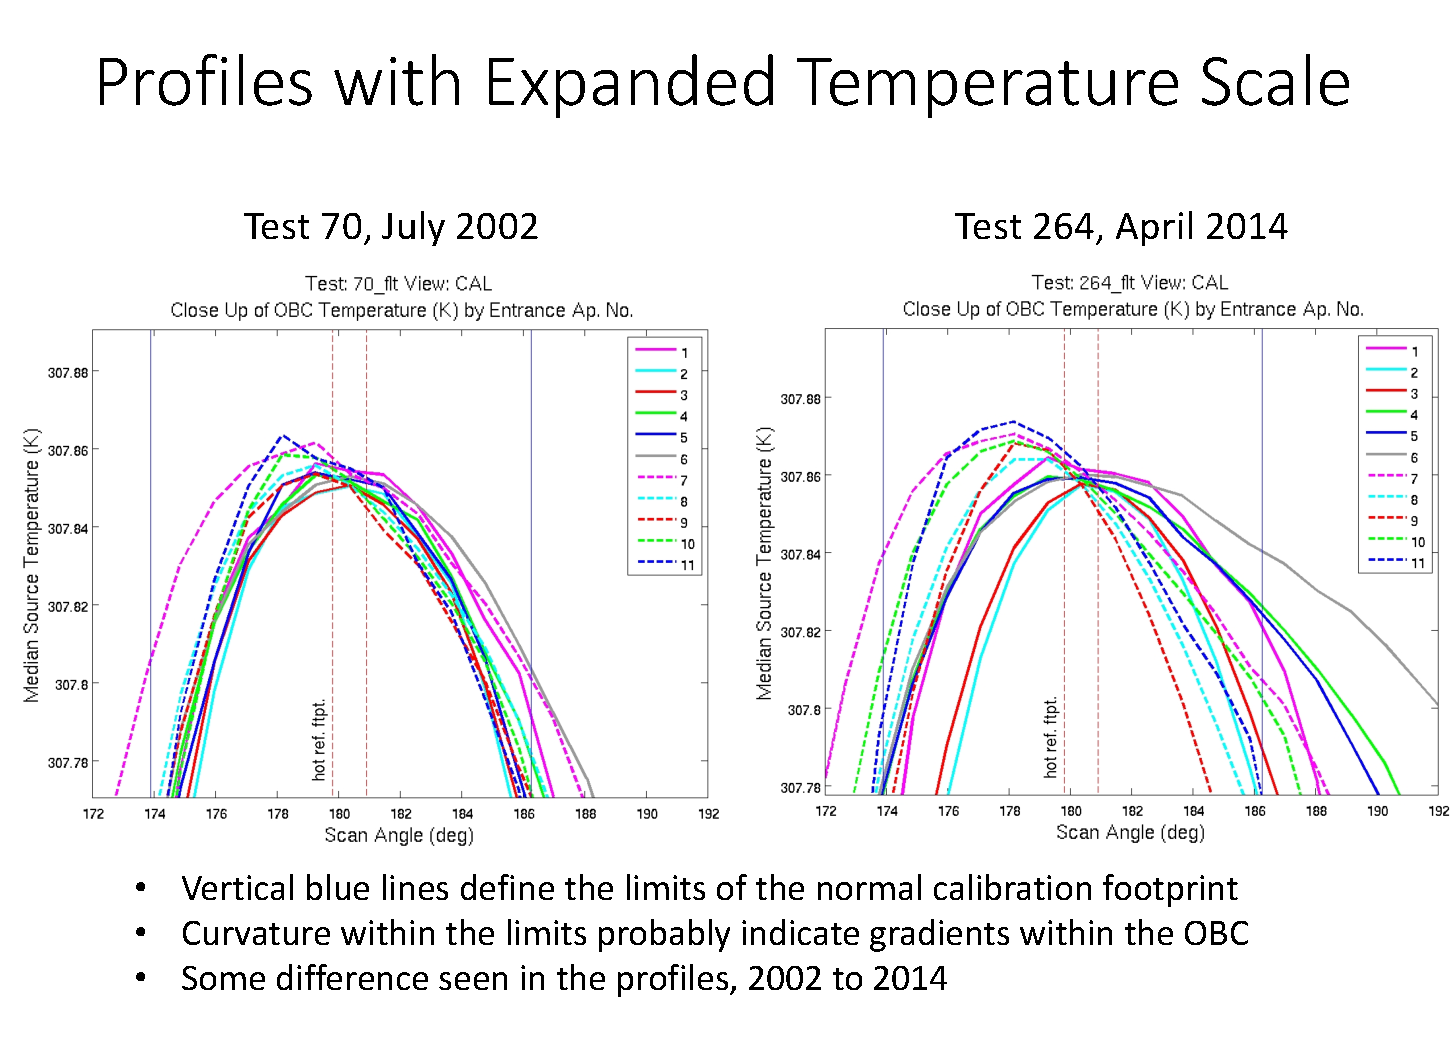
\includegraphics[width=0.8\linewidth]{./Figs/Pdf/overroye_scan.pdf}
\end{center}

\begin{small}
\begin{itemize}
\item Strongly suggests B(T) trends maybe be associated with thermal drifts over time
\item Same effects cause AIRS frequency shifts
\end{itemize}
\end{small}
\end{frame}

\begin{frame}[label={sec:orgd095c45},shrink=20]{Quick Look at Fast T\textsubscript{surface} Algorithms}
\begin{itemize}
\item Want to examine sensitivity to L1c adjustments \alert{quickly}
\item Examine channels separately
\end{itemize}

\begin{block}{Approach Presented (preliminary)}
\begin{itemize}
\item Here we generated 1231 and 2616 \wn time series from 1\% of all data
\item Gridded into lat/lon/16-day bins
\item For each 16-day bin pick the hottest BT and keep it.  So now about 0.02\% of all data
\item Form the BT anomalies for each bin and retrieve linear slope (trend)
\item Compare to ERA, OISST, etc.
\end{itemize}
\end{block}

\begin{block}{Liens and Future Changes}
\begin{itemize}
\item 1231 \wn needs dBT/dT\textsubscript{surf} adjustment (used mean values from ERA)
\item Additional adjustment needed if \water varies significantly (not done)
\item Picking hottest only is quite a small subset.
\item In future use all data, not 1\% random subset (done) and use more than just hottest scenes
\item Pick up enough full-spectrum data to fit for \water trends for 1231 \wn adjustments
\end{itemize}
\end{block}
\end{frame}

\begin{frame}[label={sec:orgbae84f2}]{Surface T Trends Using 1231 \wn Channel}
\vspace{-0.35in}

\begin{columns}
\begin{column}{0.55\columnwidth}
\begin{block}{\footnotesize AIRS 1231 \wn}
\vspace{-0.1in}
\begin{center}
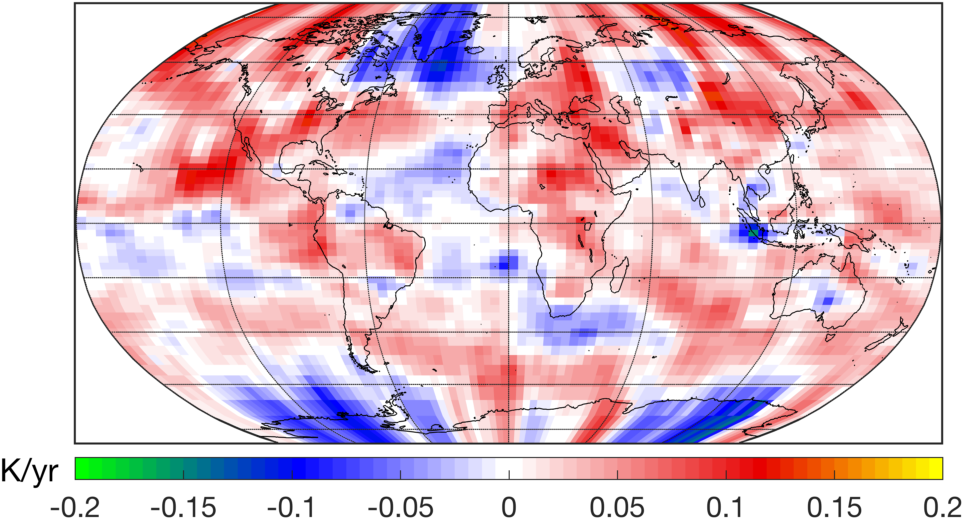
\includegraphics[width=\linewidth]{./Figs/Png/airs_tsurf_trend_from_1231cm_trend.png}
\end{center}
\end{block}
\end{column}

\begin{column}{0.55\columnwidth}
\begin{block}{\footnotesize ERA}
\vspace{-0.1in}
\begin{center}
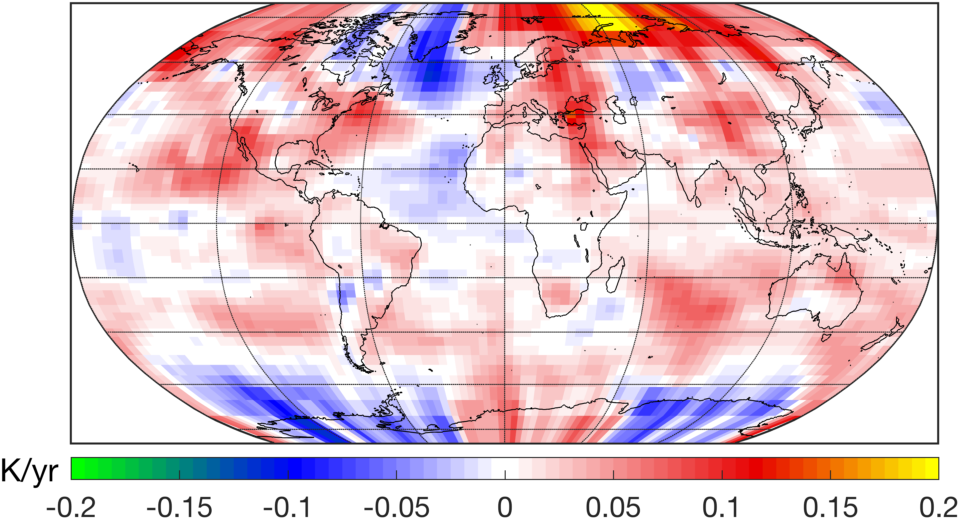
\includegraphics[width=\linewidth]{./Figs/Png/era_tsurf_trend.png}
\end{center}
\end{block}
\end{column}
\end{columns}


\begin{columns}
\begin{column}{0.55\columnwidth}
\begin{block}{\footnotesize OISST}
\vspace{-0.1in}
\begin{center}
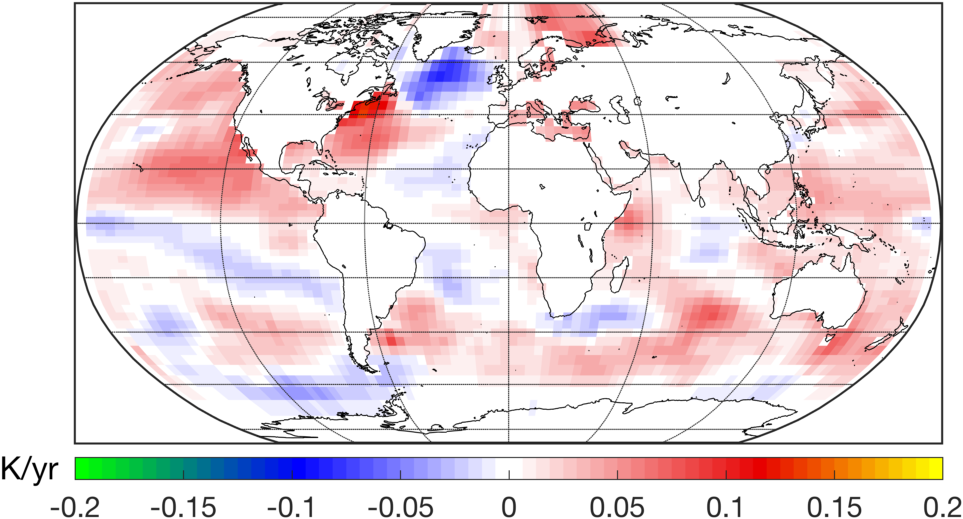
\includegraphics[width=\linewidth]{./Figs/Png/oisst_trend_map.png}
\end{center}
\end{block}
\end{column}

\begin{column}{0.5\columnwidth}
\begin{block}{\footnotesize AIRS 2616 \wn}
\vspace{-0.1in}
\begin{center}
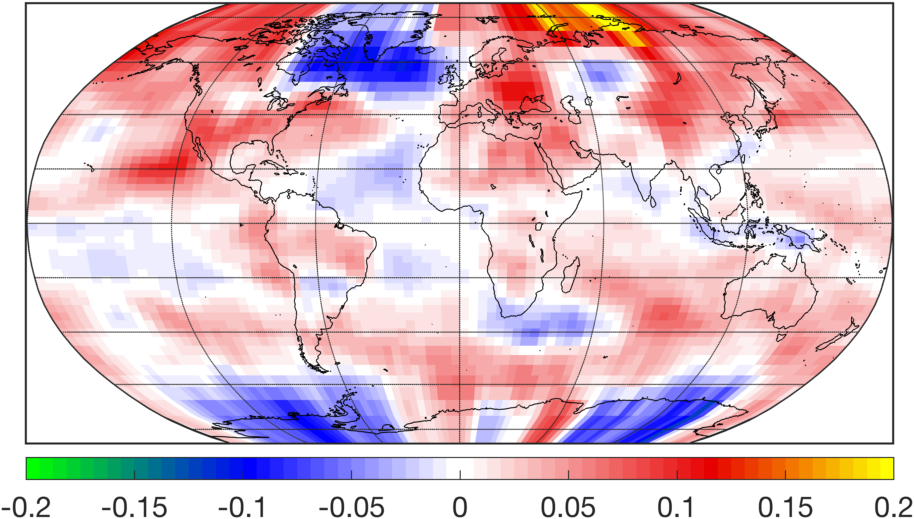
\includegraphics[width=\linewidth]{./Figs/Png/airs_tsurf_trend_from_2616cm_trend.png}
\end{center}
\end{block}
\end{column}
\end{columns}
\end{frame}

\begin{frame}[label={sec:org1355945}]{SST Trends of Previous Mapped Data (1231 \wn only)}
\begin{center}
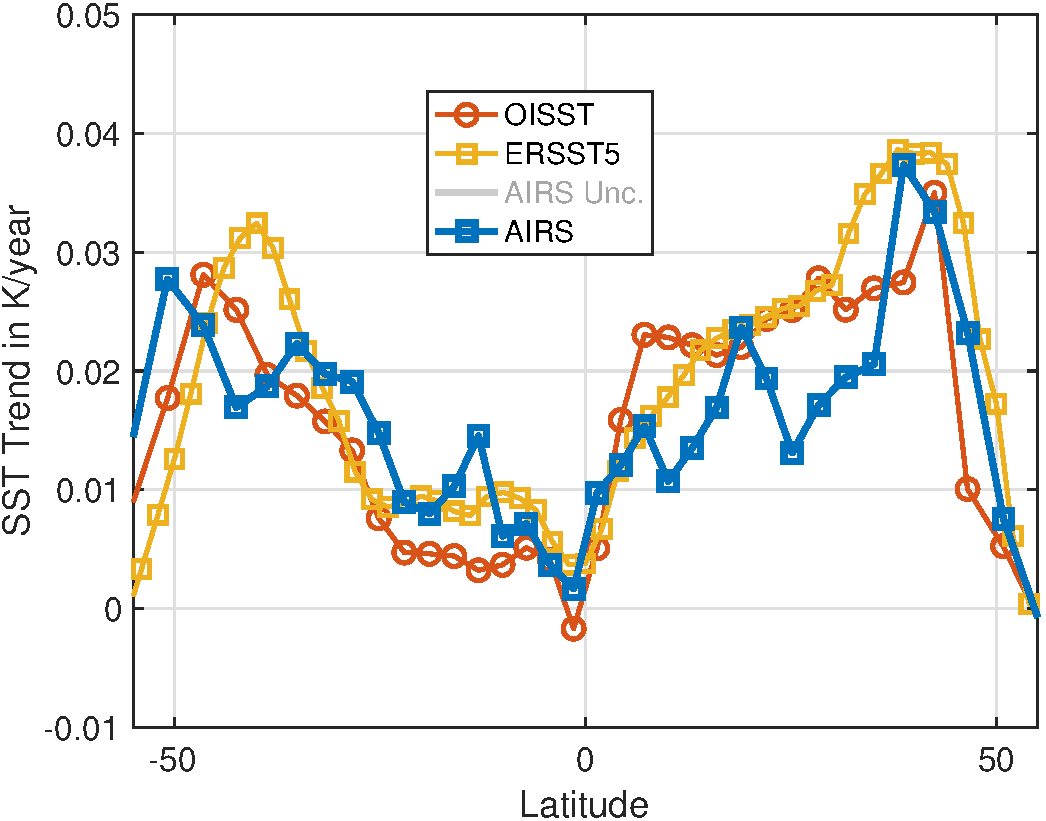
\includegraphics[width=0.7\linewidth]{./Figs/Pdf/zonal_sst_trends_12311_vs_oisst_ersst5_hottest_per_grid_envelope.pdf}
\end{center}

\begin{footnotesize}
\begin{itemize}
\item ERSST5 is considered one of the best climate surface T products
\item ERA is NOT a measurement, but sure is good!
\item Will expand to HADCRUT, GISTEMP, etc. in the future
\end{itemize}

Results appear to be quite good! 
\end{footnotesize}
\end{frame}

\begin{frame}[label={sec:org286d8ac}]{Conclusions}
\begin{itemize}
\item We have a tremendous instrument, with a very stable blackbody reference
\item But, small thermal shifts in the grating system produce BT trends that can vary with channel
\item Cold (space look) measurements appear to be the culprit?
\item The approach to fixing these problems seems doable, but will require a significant effort
\item Most climate questions can be answered if the radiometric trends are fixed
\item Better absolute radiometry will not impact most science we need to do, it's already quite good!
\item This works needs to be done now before Level 2 is used too much for climate research!
\end{itemize}
\end{frame}
\end{document}